\documentclass[12pt,a4paper]{report}
\usepackage[left=25mm, right=25mm, top=25mm, bottom=25mm]{geometry}
\usepackage[english]{babel}
\usepackage[latin1]{inputenc}
\usepackage[T1]{fontenc}
\usepackage{lettrine}
\usepackage{pslatex}
\usepackage{fancyhdr}
\usepackage{minitoc}
\usepackage{setspace}
\usepackage{url}
\usepackage{graphicx}
\usepackage[export]{adjustbox}
\usepackage{pifont}
%\frenchbsetup{StandardLists=true}
\usepackage{enumitem}
\usepackage{amssymb}
\usepackage{color}
%\usepackage{colortbl}
\usepackage{listings}
\usepackage{listingsutf8}
\usepackage{lscape}
%\usepackage{lettrine}
%\usepackage{setspace}
\usepackage{multirow}
\usepackage{marvosym}
\usepackage{textcomp}
\usepackage{lastpage}
\usepackage{hyperref}
\usepackage{pdfpages}
\usepackage{nopageno}
\usepackage{slantsc}
\usepackage{array}
\usepackage{amsmath}
\usepackage{makeidx}
\usepackage{glossaries}
\usepackage{lipsum}
\usepackage{appendix}
\usepackage[Lenny]{fncychap}
\usepackage[grey,utopia]{quotchap}
%\usepackage[colorlinks=false,linkbordercolor=white]{hyperref}
%\frenchbsetup{StandardLists=true}
%\definecolor{light-gray}{RGB}{128,128,128}
%\definecolor{light-or}{RGB}{0,0,0}
%%\newcommand\nomChap[1]{\def\@nomChap{#1}}
%\bibliographystyle{plain}
%%\bibliographystyle{unsrt}
%\makeindex
%\makeglossaries
\onehalfspacing
%*************REDENIR sommaire chapter*****************
 
\renewcommand{\thechapter}{\Roman{chapter}}

\mtcselectlanguage{english}
\begin{document}
\dominitoc
\setcounter{tocdepth}{4}
\setcounter{secnumdepth}{4}
\pagenumbering{roman} \setcounter{page}{1}
\vspace*{1cm}
 \thispagestyle{empty}
 \begin{center}
 {\fontfamily{anttlc}\selectfont{{\Huge \textbf{Dedication}}}}
 \end{center}
 \vspace*{1cm}

\fontfamily{anttlc}\selectfont{{\LARGE \textit{I}} dedicate my report work to my family. I want to express my sincere gratitude to my loving parents, Mhamed and Amel Rhaiem whose without their support and their words of encouragement it would not have been possible. \\

{\Large \textit{M}} y sister Ameni, and my brother Wajdi who have never left my side and always made me feel very special, I can't imagine my life without them.\\

{\Large \textit{I}} also dedicate this dissertation to Freeways ISI and Mozilla-Tunisia families whose have always supported me throughout the intership.\\

{\Large \textit{I}} also appreciate, Yaser Rabi for helping me develop my technology skills, and Sabri Bahrini for the many hours of proofreading.\\

{\Large \textit{I}} dedicate this work and give  a special thanks to all my best friends specially Atef.

\vspace*{1cm}
\begin{flushright}
\fontfamily{anttlc}\selectfont{{\LARGE Manel }}\\
 
\end{flushright}
\vspace*{1cm}
 \thispagestyle{empty}
 \begin{center}
 {\fontfamily{anttlc}\selectfont{{\Huge \textbf{ Acknowledgments}}}
 \end{center}
 \vspace*{1cm}
 

\fontfamily{anttlc}\selectfont{
{\LARGE \textit{I}} would like to express my deepest appreciation to all those who provided me the possibility to complete this report.  A special gratitude I give to my supervisor in the university, Mr. \textit{\mathscr{Fahem KEBAIR}}, whose contribution in stimulating suggestions and encouragement,  helped me to coordinate my project especially in writing this report. \\

{\LARGE \textit{I}} take this opportunity to express my profound gratitude and deep regards to my guide Professor \textit{Ramzi GUETARI }for his exemplary guidance, monitoring and constant encouragement throughout the course of this training. The blessing, help and guidance given by him time to time shall carry me a long way in the journey of life on which I am about to embark.\\

{\LARGE \textit{I}} also take this opportunity to express a deep sense of gratitude to Mr. \textit{Henri SEVERAC}, chef company , Stradefi SA, for his cordial support, valuable information and guidance, which helped me in completing this task through various stages.\\

{\LARGE \textit{L}}astly, I thank almighty, my parents, brother, sisters and friends for their constant encouragement without which this document would not be possible.

 }

 \tableofcontents
 \phantomsection
\listoffigures
\phantomsection
\listoftables
 
\renewcommand{\footrulewidth}{0.4pt}
\renewcommand{\headrulewidth}{0.4pt}
\renewcommand{\baselinestretch}{1.6}
 
\fancyfoot[L]{\footnotesize{\textit{Manel Rhaiem}}}	
\cfoot{}
 
\rfoot{\bf \footnotesize \thepage/\pageref{LastPage}}
\lhead{}

 
 
\pagenumbering{arabic} \setcounter{page}{1}

\chapter*{Introduction}
\phantomsection
%\addcontentsline{toc}{chapter}{Introduction}
\addstarredchapter{Introduction}
 \pagestyle{fancy}
 \thispagestyle{\renewcommand{\headrulewidth}{0pt}}
\rhead{}
\lettrine[lines=2,lhang=0.44,lraise=0,loversize=0.08,findent=-0.11em,slope=0.6em]%
{I}{} ncreasingly, data is viewed as the lifeblood of organizations. Across industries, information is sliced, diced and analyzed for trends, anomalies and insights that lead to better outcomes and strategies . In support of this, more and more organizations have adopted business intelligence (BI) solutions that help them fully capitalize on data at their fingertips. 
\paragraph*{}
Business Intelligence is the process of transforming raw data into meaningful information to enable more effective business insight and decision-making 
In fact, according to Gartner, the worldwide market for BI platforms, analytics and performance management software market grew to \$12.2 billion in 2011. Moreover, a recent Gartner survey found that CIOs list BI and analytics technology as their N� 1 priority for 2012.
\paragraph*{}
It's no surprise that these BI tools are increasingly used in conjunction with enterprise applications such as customer relationship management, enterprise resource planning and enterprise asset management, to name a few. By applying an analytics layer to these mission-critical applications, organizations derive greater value from the data they gather. Plucking new insights from and making more use of the data at their disposal helps businesses boost the ROI on these significant investment.
\paragraph*{}
BI software allows therefore companies to tap into their many databases and deliver easy-to-comprehend insights to employees, management and business partners.
Far from mere "eye candy," data visualization is critical to fulfilling widely held goals for expanding organizations? analytics culture and driving more decisions with data. Across organizations, employees who are subject matter experts in areas such as marketing, customer service, online engagement, finance, and more need to interact with data and analyze it for significant patterns, trends, and anomalies.
\paragraph*{} 
Yet, most of these professionals would hardly consider themselves "business intelligence users", much less professional data scientists or data analysts. Tools and practices for data visualization, data discovery, and visual analysis are enabling these "nontechnical" users to make effective use of data and reduce their time to insight.
Data visualization sits at the confluence of advances in technology, the study of human cognition and perception, graphical interfaces, widespread adoption of standards for rich Internet applications, and the continuing expansion of interest and experience in analytics and data discovery. Data visualization can contribute significantly to the fruitful interpretation and sharing of insights from analytics, enabling nontechnical SMEs to perform data discovery in a self-directed fashion. 
\paragraph*{}
Implementation of chart engines and the growth in the number and variety of visualizations available in graphics libraries are supporting new sophistication in visual analysis, allowing users to go beyond simple bar and pie charts to express more advanced insights about quantitative information.
\paragraph*{}
Stradefi SA is one of these companies that has found out that strong data visualization and graphical discovery analysis are essential for its customer to realize benefits from large, complex, and diverse data volumes. It aims to provide its customers and partners with easy-to-use graphical interfaces for accessing and analyzing data. Now, sophisticated charts enable users to advance their understanding. They can discover hidden data relationships within a range of internal and external sources, including geospatial data, and improve self-service actionable insight. 
\paragraph*{}
The $IG�$ software application that is being developed is one of the BI oriented systems dedicated to data visualization. it allows to represent a complex set of data bound to each other as a graph data structure that facilitates the comprehension, the management and the modification of each datum and its relations. The $IG�$ software is intended to be able to visualize complex data (the objects and their relations) on different devices, especially mobiles ones.
\paragraph*{}
This document presents the solution that I have developed in response to the specifications provided by Stradfi SA that present the business requirements. It is organized in five chapters. The chapter one concerns the problem statement. It presents how is born the idea of the bounded data visualization and the development if $IG�$ were born. The chapter two presents the state of the art and also discusses the solutions that have been chosen to develop the application. The chapter three the feasibility analysis and the requirements determination. The chapter four discusses the project plan and monitoring. And, finally, the chapter five discusses the realization of the prototype of the $IG�$.
\phantomsection
\renewcommand{\thepage}{}
\chapter{Problem Statement}
\thispagestyle{empty}
\pagestyle{fancy}
\lhead{\small \bf  Chapter 1: Problem Statement}
\rhead{}
\chead{}
\renewcommand\thepage{\arabic{page}}
 \setcounter{minitocdepth}{1}
\minitoc
 
\newpage
\section{Introduction}
\lettrine[lines=2,lhang=0.44,lraise=0,loversize=0.08,findent=-0.11em,slope=0.6em]%
{I}{} nformation is always the critical success factor of key of strategic decisions. The fast growing market of mobile devices as smart phones and tablets changes drastically the picture and offer new way of working. These mobile devices overwhelm the population and might become the preferred computing tools. Information becomes mobile.
The increased use of mobile computing has imposed a new challenge: the ability to represent information of any kind on smaller devices. It is in this context that the idea of radial representation of data structures organized as trees and graphs is born. The company Stradefi-SA, which we present in the following paragraph, had an urgent need to achieve a 3-tier architecture based application capable of managing data organized in the form of graphs and trees.
This application, which is intended for an intensive use by intermediate of mobile devices, must support the radial representation of these
data structures.
  
\section{Company's presentation}
\paragraph*{}
\textbf{Stradefi-SA} is a privately owned company in Geneva specialized in highly secured. It servers the content management, Business process and customer relation. Works in private Cloud Mobile Computing architecture. Stradefi`s consultants delivered innovative solution to companies as:Novartis, PNB PARIBAS, Romande Energie
\section{Project issues}
\paragraph*{}
In the real life a lot of relationships exist between different entities. An entity may be a physical person or any kind of object. These relations may be unilateral, bilateral, or multiple. Every single object could have relations with hundreds of other entities.
\paragraph*{}
To automate the management of entities and their relationships, and in order to process them by computers, one must represent them as abstractions. One of the most active areas in the IT domain is "Graph and Tree" representation [1]. In the Graph Theory, a Graph is a representation of a set of objects where some pairs of objects are connected by links.
\paragraph*{}
Formally, a Graph [1] is a pair G = (V, E) of sets, where V is the set of vertices, such that $E = [V]�$ formed by pairs of vertices. formed by pairs of vertices. E is a multiset, in other words, its elements can occur more than once so that every element has a multiplicity [2].
\paragraph*{}
A directed graph (or digraph) [W3] in mathematics, and more specifically in graph theory,is a graph, or set of nodes connected by edges, where the edges have a direction associated with them. A set V, whose elements are called vertices or nodes, and a set E of ordered pairs of vertices, called arcs, directed edges, or arrows (and sometimes simply edges with the corresponding set named E). It differs from an ordinary or undirected graph, in that the latter is defined in terms of unordered pairs of vertices, which are usually called edges. This(figure-1) illustrate a Directed Graph:
\vspace*{2mm}
\begin{figure}[h]
\begin{center}
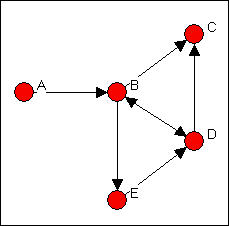
\includegraphics[scale=0.5, frame]{Figure_1.jpg}
\end{center}
\caption{Directed Graph}
\end{figure}
\paragraph*{}
In the theory there is no restrictions on the number of relations that a certain node may have.
Depending on the piece of the displayed graph, the node may appear disconnected as illustrated in (figure-2):
\begin{figure}[h]
\begin{center}
\includegraphics[scale=0.5]{tel11.png}
\end{center}
\caption{Usual graphical representation of a graph/tree}
\label{Figure of Simple Graph Representation}
\end{figure}
\paragraph*{}
The work that has been achieved is intended to manage the presentation of Graph in a way that avoids the problems described above.
\section{Project summary}
\paragraph*{}
Customers of \textbf{Stradefi SA} usually are Pharmaceutical Laboratories, Private Banks, Medical Cabinets, etc. This kind of organizations manage lots of entities as well as relationships between them. For example a customer of a private bank may have different accounts of different types.
\paragraph*{}
He also may have some bank advisers. He may have a shared account with his wife, etc. The customer, his wife, the adviser and the different account are seen as entities that are bound by relationships:
\begin{itemize}
\item the customer owns the accounts,
\item the customer has a wife,
\item the customer is advised by a bank employee,
\item etc.
\end{itemize}
\paragraph*{}
It is, therefore natural to abstract and represent the entities and their relations in the form of Graphs as we have already mentioned that in the introduction. The work present on this report is to implement an application that covers the need to manage entities that have relations with each other and implemented in the form of Graphs. We have identified through a technical interview with the customers, and from there business our objectives.
\subsection{Proposed solution}
\paragraph*{}
Referring to the issues that have been exposed in $�1.3$ the classical visualization of graphs and trees is not suitable to mobile devices. We, therefore, have investigated other kinds of these data structures visualization that combine simplicity and efficiency. We found out that the radial representation is the solution to these issues. 
\paragraph*{}
The radial layout encodes directed graphs on narrow rings of a circle [3]. The hierarchical evolution of the graph is mapped to rings that grow outward from the center of the circle. Graph vertices are placed equidistantly at the borderlines of each ring. Graph edges are displayed as curved lines starting from a source on the inner borderline of the ring and pointing to a target on the outer borderline. To better perceive link directions and structures of large data-sets, visual clutter is reduced by exploiting an edge splatting approach that generates density felds of the displayed edges. The radial layout emphasizes newer graphs, displayed in the larger, outer parts of the circle. As a benefit, edge lengths are reduced in comparison to the non-radial visualization. Moreover, the radial layout guarantees the symmetry of the visualization under shifting of vertices.
\begin{figure}[h]
\begin{center}
\includegraphics[scale=0.5]{tel22.png}
\end{center}
\caption{Radial Form}
\label{Figure of Radial Representation}
\end{figure}
\section{Conclusion}
\paragraph*{}
In this chapter we have discussed the issues related to data visualization on mobile devices, especially data that is formalized in the form of graphs and trees. We have also presented the motivation of Stradefi-SA to implement a solution that covers all of these problems. Potential customers exist and there is a real need that has been expressed trough technical interviews conducted by the company.
\paragraph*{}
The challenge was to chose between two alternatives: implement an application from the scratch or use an already existing library that is capable of the radial visualization. This will be discussed in the following chapter: "state of the art".

\renewcommand{\thepage}{}
\chapter{State of the art}
\thispagestyle{empty}
\pagestyle{fancy}
\lhead{\small \bf  Chapter 2: State of the art}
\rhead{}
\chead{}
\renewcommand\thepage{\arabic{page}}
 \setcounter{minitocdepth}{1}
\minitoc
\clearpage

\section{Introduction}
\lettrine[lines=2,lhang=0.44,lraise=0,loversize=0.08,findent=-0.11em,slope=0.6em]%
{I}{} mplementing an algorithm allowing to visualize graphs/trees data structure is a challenging but feasible task. Lots of works presenting such algorithms have already been done and published. Greg Book \& Neeta Keshary from the University of Connecticut present in [4] the implementation of an algorithm for the radial visualization of large hierarchies. Maxime Dumas at al. in [5] also present a solution for the optimization of a radial layout of bipartite graphs.
Some of these algorithms have been improved and implemented as open source solutions. The choice has therefore been easy to make. We decided to use an existing open source library instead of implementing our own algorithm.
In this state of the art, we compare different existing solutions and discuss pro and cons of each one of them in order to explain the reasons that have oriented us in our final choice.
\section{Radial representation}
\paragraph*{}
A radial graph drawing is a representation in which the vertices lie on concentric circles of finite radius. In the context of our domain, this kind of representation facilitates the management and the exploration of data structures, formalized as graphs, using mobile devices. These latter "suffer" from the usual small size of their displays.
\paragraph*{}
Many implementations of different algorithms exist [6]. Some of them have been implemented in C, others in Java, etc. According to the specification of our application, we had to implement a HTML 5 based application. We had either to implement our own visualization application or, rather use an existing open source library. As we have already mentioned it, our choice went to an open source library. In the following paragraphs we present a survey of some existing solutions in order to select the one that covers all/most of our needs.
\paragraph*{}
The use of HTML5 imposes the inherent technologies and languages to be used: HTML/XML, CSS and JavaScript. Our main objective was to select the appropriate JavaScript library that supports the radial visualization of graphs and trees. We have experimented, among others, D3JS [7][W4], JavaScript Infovis Tools (JIT) [8][9][W5] and SigmaJS [W6].
\subsection{Javascript Infovis Tools (JIT) Framework}
\paragraph*{}
The JavaScript InfoVis Tollkit (JIT) is a JavaScript information visualization library that enables interactive visualizations of data using only HTML, CSS and JavaScript. InfoVis was created by Nicolas Garcia Belmonte in 2008 and acquired by Sencha Labs in 2010[W7]. The basic idea behind using InfoVis is to first define your data, and then instantiate a new object from the selection of predefined chart types defined in InfoVis, and finally load your data into the object.
\paragraph*{}
The predefined chart types generally expect data to be JSON objects formatted in a specific way. Objects may grouped in different groups, A \textit{color} property specifies the colors that should be used for each grouping. A \textit{label} property correlates to the labels on the axes for each grouping. Finally a \textit{values} property is quite literally an array that holds objects that specify the values for each grouping.
To create a new chart in InfoVis one must instantiate a new object from the list of predefined chart types that InfoVis supports:
\begin{itemize}
\item AreaChart
\item BarChart
\item PieChart
\item TreeMap
\item Force Directed
\item \textbf{Radial Graph}
\item Sunburst
\item Icicle
\item SpaceTree
\item HyperTree
\end{itemize} 
\paragraph*{}
While this may be a limiting factor if you want to create a chart that is not yet supported, it can also be seen as an opportunity. The InfoVis project is completely open source and available on Github. To create a new chart, one needs to instantiate a new object from the constructor of the chart type needed. From the above information it should be clear that by using InfoVis you can create rich, interactive charts. InfoVis is ideal for quickly producing professional looking data visualizations. The limitation with InfoVis is if you want to use a chart type that is not yet supported, like a time series, bubble chart, or spark line.
\subsection{D3JS Framework}
\paragraph*{}
D3JS is a JavaScript library for manipulating documents based on data. That means that it is a tool that can be used in conjunction with other tools to get a job done. Those other tools are mainly HTML and CSS (amongst others) but you don't need to know too much about either to use D3. It's an open framework, which means that there are no hidden mysteries about how it does its magic and it allows others to contribute to a constant cycle of improvement. It's built to leverage Web standards which means that modern browsers do not have to do anything special to use D3, they just have to support the framework that the Internet has adopted for ease of use.
\paragraph*{}
The interesting feature of D3 is that it allows you to associate data and what appears on the screen in a way that directly links the two. Change the data and you change the object on the screen. D3 is trick is to let you set what appears on the screen. A circle, a line, a point on a map, a graph, a bouncing ball, a gradient (and way, way more). Once the data and the object are linked the possibilities are endless.
\subsection{Sigma JS Framework}
\paragraph*{}
Sigma JS is a JavaScript library dedicated to graph drawing. Sigma provides a lot of built-in features, such as Canvas and WebGL renderers or mouse and touch support, to make networks manipulation on Web pages smooth and fast for the user. It provides a lot of different settings to simplify the  customization of the drawing and the interaction with networks. It is also possible to add user functions to customize the rendering of nodes and edges.
\paragraph*{}
Sigma is a rendering engine, it, therefore allows to add the needed interactivity. The public API makes it possible to modify the data, move the camera, refresh the rendering, listen to events, etc. Sigma aims to help you display networks on the Web, from simple interactive publications of networks to rich Web applications featuring dynamic network exploration.
\subsection{Discussion}
\paragraph*{}
In this table (table-1) we present a comparative between these librairies which respond to the most of our requierements, and we explain the developement of each library 
\newpage
\begin{landscape}
\begin{table}[Ht!]
\centering
\begin{tabular}{|p{5cm}|p{5cm}|p{5cm}|p{5cm}|}
\hline
\textbf{\begin{center}
features
\end{center}}& \textbf{\begin{center}
SigmaJS 
\end{center}}& \textbf{\begin{center}
D3JS
\end{center}} & \textbf{\begin{center}
Javascript Infovis Toolkit
\end{center}}\\
\hline
Parse structured data and graphically visualize it  & yes & yes & yes \\
\hline
Render radial graph & no only usual graphs & yes & yes \\
\hline
Creation of nodes and relations from a script & yes & yes & yes\\
\hline
Creation of nodes and relations interactively & yes & no & yes \\
\hline
Remove relations & no & yes & yes\\
\hline
Update relations & no & yes & yes\\
\hline
Select Nodes & yes & yes & yes \\
\hline
Select the node of interest & no & no & yes:OOTB \\
\hline
Relations' filtering & yes & yes & yes \\
\hline
Search & no & no & no\\
\hline
Drag and Drop (Nodes, Graph) & yes & yes & yes \\
\hline
Navigate in the radial graph & yes & yes & yes \\
\hline
Access to the contain of nodes and relations & no & yes & yes \\
\hline
\end{tabular}
\caption{Summary of the graphic Javascript Librairies}
\label{Librairies comparative}
\end{table}
\end{landscape}
\paragraph*{}
This short survey has shown that SigmaJS is an interesting library however there is no support of radial visualization. At the first glance, D3JS and JIT seem close to each other and offer almost the same features and capabilities.
\paragraph*{}
D3JS doesn't allow to center the node of interest, while this feature come out-of-the-box in JIT. In the application specification, centering the node of interest is a requirement.
\paragraph*{}
There is no support of the interactive creation of nodes and edges in D3JS. In JIT it is possible to add nodes and edges using a form.
\paragraph*{}
Other minor feature differ from D3JS and JIT, however they are not that important. Thus we have chosen JIT to implement the $IG�$ application.
\section{Conclusion}
In this chapter we have presented the results of the experiments we did with some JavaScript graphical libraries. Except SigmaJS, the other libraries are suitable to the specifications. Both D3JS and JIT allow the radial representation of data structures in general and graph in particular. The choice of JIT has been oriented by some out of the box characteristics that are not supported in D3JS and need an additional effort in order to implement them.

\renewcommand{\thepage}{}
\chapter{Feasibility Analysis and Requirements Determination}
\thispagestyle{empty}
\pagestyle{fancy}
\lhead{\small \bf  Chapter 3: Feasibility Analysis and Requirements Determination}
\rhead{}
\chead{}
\renewcommand\thepage{\arabic{page}}
 \setcounter{minitocdepth}{1}
\minitoc
\clearpage
\section{Introduction}
\lettrine[lines=2,lhang=0.44,lraise=0,loversize=0.08,findent=-0.11em,slope=0.6em]%
{T}{} he $IG�$ application is intended to be used by various businesses, and especially pharmaceutical companies, private banks and medical offices. It has therefore been conceived to meet the needs of each business to which it is addressed. The majority of the needs are common to all kinds of usage, however specific ones depend on each business. Our application has been designed and developed to be open and configurable enough to adapt to the businesses for which it was tested as well as other.
\paragraph*{}
A specification is the definition of the project: a statement of the problem, not the solution. Normally, the specification contains errors, ambiguities, misunderstandings and enough rope to hang you and your entire team. Thus before embarking upon a long time of activity working on the wrong project, one must assume that a numbty\footnote{a numbty is a person whose brain is totally numb. In this context, numb means "deprived of feeling or the power of unassisted activity"; in general, a numbty needs the stimulation of an electric cattle prod to even get to the right office in the morning. Communication with numbties is severely hampered by the fact that although they think they know what they mean (which they do not), they seldom actually say it, and they never write it down. And the main employment of numbties world-wide is in creating project specifications. You must know this - and protect your team accordingly.} was the chief author of the received specification and one must read, worry, revise and ensure that everyone concerned with the project (from originator, through the workers, to the end-customer) is working with the same understanding. The outcome of this deliberation is a written definition of what is required, by when; and this must be agreed by all involved.
\paragraph*{}
The work on the specification can be seen as the first stage of Quality Assurance since one is looking for and countering problems in the very foundation of the project - from this perspective the creation of the specification clearly merits a large investment of time. From a purely defensive point of view, the agreed specification also affords a protection against the numbties who have second thoughts, or new ideas, half way through the project.
\section{Identification of the business requierements}
\paragraph*{}
The specifications have been provided by The Stradefi-SA team and discussed with the appropriate persons. After analyzing the specifications, we identified the following business requirements:
\begin{itemize}[font=\color{black}, label=\ding{98}]
\item The nodes can be individuals, objects or any abstract entity.
\item The edges represent relationships between the nodes. These relationships can be unilateral, bilateral or double.
\item Nodes as well as relations have properties and attributes. The application populates the necessary properties attached to the nodes and edges for the radial representation of the information received from the JSON files.
\item Nodes and relations are specified in JSON file. The use of XML is possible in order to make the $IG�$ Application open to other usages and other businesses.
\item The application explores the JSON files, identifies the nodes and relationships and builds a radial graph.
\item The nature of the relationship (unilateral, bilateral or multiple) is a characteristic that the application is able to analyze and represent.
\item Documents may  be associated to nodes (underlying document). They are stored in a document management system. The document path or ID is a property of the node.
\item When a node is selected it becomes the node of interest. It is automatically centered (becomes the center of the radial graph).
\item Some (significant) properties related to a given node, can be shown in a Panel, when the node is clicked.
\item A relation might be described in a document (underlying document). The document is therefore associated to the relation and stored in a document  management system. The document path or ID is a property of the relation.
\item The application calculates the distance between nodes. Distance defines, for instance, the degree of relation between two persons. The distance is defined with a level (it is anticipated that five levels are sufficient):
\begin{itemize}[font=\color{black}, label=\ding{227}]
\item Level 1 means that the two nodes are directly connected.
\item Level 2 means that the two nodes are connected via and 3rd node.
\item Etc.
\end{itemize}
\item The application is able to organize and arrange the nodes on the appropriate orbits.
\item The $IG�$ application allowing navigating through the radial graph:
\begin{itemize}[font=\color{black}, label=\ding{227}]
\item By double clicking on a node, an extra menu appears with extra feature:
 \begin{itemize}
  \item Display property in an extra pane
  \item Make this node as "selected", this action redraws the graph.
  \end{itemize}
\end{itemize}
\item Showing Mouse over (mouse only) the node or over the relation displays the property of the object (either in pop up or in another window)
\item A "mouse click" (touch also) makes the display permanent until a close on the top right cross.
\item A "double click" (touch again) opens the underlying document (click on the node, click on the relation).
\item The document opens in a separate Web onglet.
\item The user can create a graph in two ways:
	\begin{itemize}[font=\color{black}, label=\ding{227}]
	\item Scriptural: he fills a form with fields, drop down list...
	\item Graphical: capability to draw a line on a graph to create a relation, key in the properties and attaching documents
	\end{itemize}
\item The document is attached to the relation. If the document is uploaded from the PC, the document is loaded to the content management implying metadata to be filled manually or automatically
\item The user is able to change the display of nodes and edges upon their own properties.
\item The user can save a graph and its setting. 
\end{itemize}
\section{Analysis of business requirements}
\paragraph*{}
The business requirements presented in the last paragraph are the result of several discussions that we had inside the team. The specifications of the $IG�$ application expressed lots of requirements however we considered only some of them that seemed to us the most significant ones. For the detailed list of selected requirements, please refer to the table IV.1. These final requirements was considered as the product backlog and we started the design and the implementation if the $IG�$ application on the basis of this backlog. In this chapter we present the different use cases and activity diagrams corresponding to the items that have been developed in the current version of $IG�$.
\subsection{The general Use Case}
\paragraph*{}
The following diagram represents the overall view of $IG�$ application. The user can create a new graph or act on an existing one. He can select a node in order to move it, to access to its properties and attributes and  to update them. The user can select a relation, to see its properties and to modify them. 
\newpage
\begin{figure}[h]
\centering
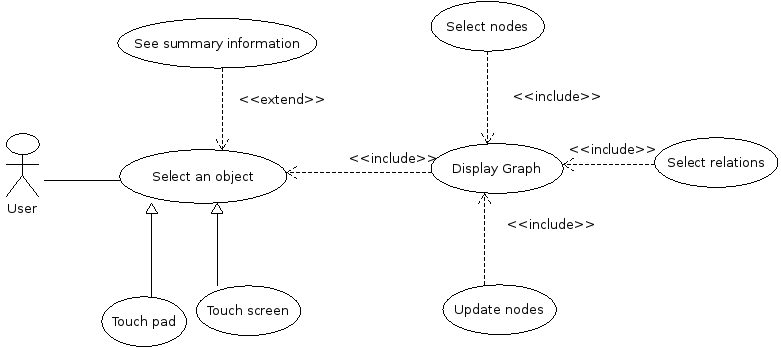
\includegraphics[scale=0.75, frame]{GeneralUseCase.png}
\caption{General use case diagram}
\end{figure}
\subsection{Use Case: Display a Graph}
\paragraph*{}
This functionality allows the end user to visualize his object and their relationships by rendering a radial graph.
\begin{itemize}[font=\color{black}, label=\maltese]
\item A user interface dialogue allows to select an object, in order to display the corresponding Radial Graph;
\item When the mouse cursor goes over an object, a summary of its information is shown in a tooltip;
\item By selecting an object, the corresponding Radial Graph is displayed.
\end{itemize}
\newpage
\subsubsection{Use Case description}
\begin{table}[h]
\begin{tabular}{|p{5cm}|p{10cm}|}
\hline
\textbf{Title} & Display Graph\\
\hline
\textbf{Actor} & User\\
\hline
\textbf{Pre condition} & The user must be logged in and the list of the objects he can access to, is not empty.\\
\hline
\textbf{Post Condition} & This step ends when the Graph is displayed\\
\hline
\textbf{Description} & \begin{itemize}
\item The list of the available objects, that the user can access to, is shown in a dialog.
\item By passing the mouse cursor over an object a summary of its properties is shown.
\item the user selects an object by clicking on it and the corresponding radial graph is displayed
\item the user can access, either  to the summary of the properties of any node or the detailed attributes of the node of interest
\end{itemize} \\
\hline
\end{tabular}
\caption{textual description }
\label{Textual description}
\end{table}
\subsubsection{Use Case diagram}
\paragraph*{}
The figure III.2 presents the detailed use case diagram of the document visualization module.
\begin{figure}[h]
\begin{center}
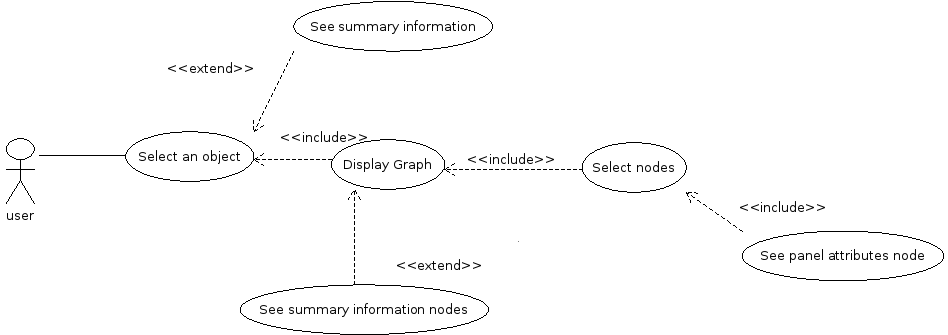
\includegraphics[scale=0.6, frame]{DisplayGraphUC.png}
\end{center}
\caption{Display Graph Use Case}
\end{figure}
\subsubsection{The "Display Graph" activity diagram}
\paragraph*{}
The user connects to $IG�$ application, the different objects  he can access to are listed in the screen.
The list may be empty if the user has no access rights to any object. If the list is not empty, he can select an object and visualize the corresponding radial graph. The default node of interest is centered. The user may select a different node that becomes the new node of interest and therefore centered. He can access, either  to the summary of the properties of any node or the detailed attributes of the node of interest.
\begin{figure}[h]
\begin{center}
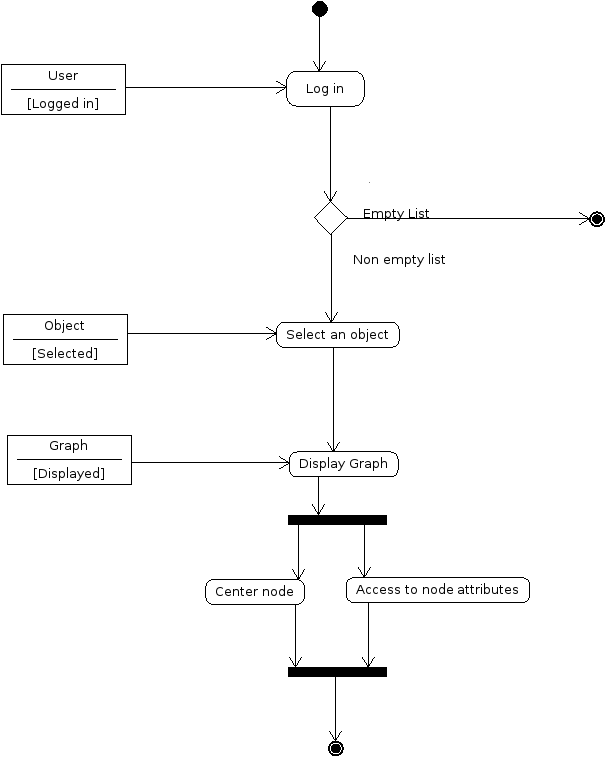
\includegraphics[scale=0.8, frame]{DisplayGraphAD.png}
\end{center}
\caption{Display Graph Activity Diagram}
\end{figure}
\newpage
\subsubsection{Use Case: Update Node}
\paragraph*{}
This use case allows users to change or update a given node proprieties\\
\begin{table}[h]
\begin{tabular}{|p{5cm}|p{10cm}|}
\hline
\textbf{Title} & Update nodes \\
\hline
\textbf{Actor} & User \\
\hline
\textbf{Pre Condition}& Only the node the interest may be updated. The user must be logged in \\
\hline
\textbf{Post Condition} & This step ends when the user comfirms or cancels the modification\\
\hline
\textbf{Description}& The user selects "modify node" menu item. The detailed attributes of the node of interest are shown in a popup window. He, then can modify one or more attributes. The updating of attributes may be confirmed or canceled.\\
\hline
\end{tabular}
\caption{textual description "Update Nodes"}
\label{Textual description of update nodes}
\end{table}
\subsubsection{Use Case diagram }
\begin{figure}[h]
\begin{center}
\includegraphics[scale=0.8, frame]{UpdateNodesUC.png}
\end{center}
\caption{Use case Update node}
\end{figure}
\subsubsection{The "Update Nodes" Activity Diagram}
\paragraph*{}
The activity diagram (fig. 3.8) details the "node update use case". The user must be connected, then he selects the "update node" item in the general menu. This item applies only on the node of interest and displays its attributes. Each attributes is put in an input text that the user may modify. After updating the appropriate attributes the user can save his modifications or cancel the operation. The confirmation of the actions results in the updating of the JSON file.
\newpage
\begin{figure}[h]
\begin{center}
\includegraphics[scale=0.8, frame]{UpdateNodesDA.png}
\end{center}
\caption{Node Update Activity Diagram}
\end{figure}
\section{Conclusion}
\paragraph*{}
This chapter results from the detailed analysis of the specifications given by Stradefi SA. The business requirements have been clearly identified and validated. Each requirements has been specified and designed. We therefore presented a use case and an activity diagram for the most important requirements. Each of them has also been validated with Stradefi SA. Some of the requirements were not completely expressed and one decided to delay their analysis and design; this will be detailed in the next chapter that discusses the methodology and the project plan.


\renewcommand{\thepage}{}
\chapter{The project plan}
\thispagestyle{empty}
\pagestyle{fancy}
\lhead{\small \bf  Chapter 4: The project plan}
\rhead{}
\chead{}
\renewcommand\thepage{\arabic{page}}
 \setcounter{minitocdepth}{1}
\minitoc
\clearpage
\section{Introduction}
\lettrine[lines=2,lhang=0.44,lraise=0,loversize=0.08,findent=-0.11em,slope=0.6em]%
{T}{} he work that has lead us to achieve the application has been managed as a project. To be successful a project must:
\begin{itemize}[font=\color{black}, label=\maltese]
\item Deliver the outcomes and benefits required by the organization, its delivery partners and other stakeholder organizations;
\item Create and implement deliverables that meet agreed requirements;
\item Meet time targets;
\item Stay within financial budgets;
\item Involve all the right people;
\item Make best use of resources in the organization and elsewhere;
\item Take account of changes in the way the organization operates;
\item Manage any risks that could jeopardize success;
\item Take into account the needs of staff and other stakeholders who will be impacted by the changes brought about by the project.
\end{itemize}
\paragraph*{}
In order to manage effectively it helps to understand the typical lifecycle of a project and how it applies to our specific one. One needs to decide how the management activities of the lifecycle steps will be achieved, and precisely who will be involved. One must make sure he understands his role in making these things happen in the right way and at the right time.\\
Much of the project management effort across the lifecycle are driven by the owner/sponsor of the project (known as the Senior Responsible Owner (SRO) ), and the Project Manager. To achieve success they will almost certainly need to draw upon the skills and experience of many others from within the organization, its partners and suppliers.
\begin{figure}[h]
\centering
\includegraphics[scale=0.6, frame]{p-lifecycle.jpg}
\caption{The project life cycle}
\end{figure}
\paragraph*{}
While Step 3 - Running a Project is by far the most resource intensive part of the project, it is the care and effort devoted to project start up and initiation that makes the most significant contribution to project success. The success of a project critically depends upon the effort, care and skill one applies in its initial planning.
\paragraph*{}
In this chapter we present the methodology adopted for the development, thereafter we explain our progress work and we wind up with the backlog Product.
\section{Methodology and software development life cycle}
\paragraph*{}
Managing a project requires a precise methodology that depends on its size and type. For small projects that the domain is well known, a Waterfall life cycle [W8] is very suitable.
All of the business requirements are well known from the beginning of the project and the Waterfall life cycle is able to handle requirements that are intended to extend the project. When the domain of interest of the project is mastered and if its size is important one must rather use a V-model life cycle[W9]. If all of the requirements are not well known or some of them are unclear, an iterative life cycle [W10] is mandatory.
\paragraph*{}
Stradfi SA has clearly expressed that all of the requirements are not clearly defined and some of them may change. Thus we agreed on the usage of an iterative life cycle. Since the team involved in the development of the $IG�$ application is small and there one have decided a daily communication about the progress of the project and the issues encountered, the SCRUM [W11] methodology becomes the best choice. 
\subsection{SCRUM's presentation}
\paragraph*{}
Agile software development processes are influenced by best practices in Japanese industry, particularly by lean development principles [10] implemented at companies like Toyota [11] and Honda [12], and knowledge management strategies developed by Takeuchi and Nonaka [13], now at the Hitotsubashi Business School in Japan, and Peter Senge [14] at MIT. Scrum is an Agile methodology that delivers software to customer and end users faster, better, and cooler [15] [16].
\paragraph*{}
Scrum works because it optimizes the development environment, reduces organizational overhead, and closely synchronizes market requirements with early feature delivery. Based in modern process control  theory, Scrum produces the best possible software given the available resources, acceptable quality levels, and required release dates. At its core, Scrum is an iterative, incremental process for developing any product or managing any work that produces a potentially shippable set of functionality at the end of each iteration. Scrum's attributes are:
\begin{itemize}
\item Scrum is an agile process to manage and control development work.
\item Scrum is a wrapper for existing engineering practices.
\item Scrum is a team-based approach to developing systems when requirements are changing rapidly.
\item Scrum controls the chaos of conflicting interests and needs.
\item Scrum improves communication and maximizes cooperation.
\item Scrum detects and removes anything that gets in the way of developing and delivering products.
\item Scrum is a way to maximize productivity.
\item Scrum scales from single projects to entire organizations, and has managed development for multiple interrelated products and projects with over a thousand team members.
\item Scrum is a way for everyone to feel good about their job, their contributions, and know they have done the very best they possibly could.
\end{itemize}
\paragraph*{}
The method is characterized by the production of a Product Backlog where requested features are organized by their priority (Figure IV.2). A Product Owner is responsible for approving changes to the product backlog. Implementation occurs in roughly 30 day iterations called Sprints which focus on the top priorities in the Product Backlog. The goal of each Sprint is to deliver a potentially shippable product increment. During the Sprint, checkpoints are observed in a daily "Scrum" meeting which communicates the progress and activities within the team and shares issues that may be "blocking" progress for an individual or the team. This allows the Scrum Master to determine progress against the Sprint commitments and advise on midcourse corrections to assure successful completion of the Sprint.
\newpage
\begin{figure}[h]
\begin{center}
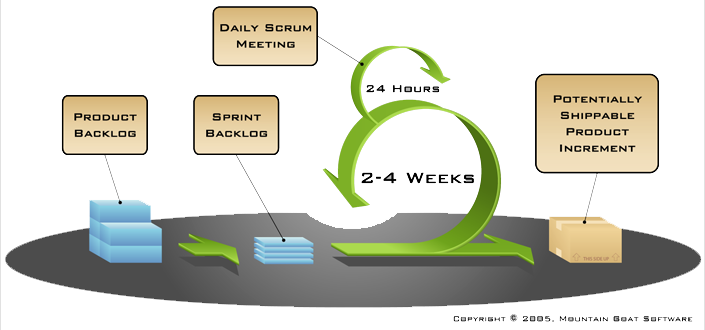
\includegraphics[scale=0.5, frame]{cycle-scrum.png}
\end{center}
\caption{The Scrum process}
\end{figure}
\subsubsection{Scrum Principles}
\paragraph*{}
While those are some of the mechanics of Scrum, more importantly, one should understand that Scrum is guided by a few key principles: 
\begin{itemize}
\item The belief that effective software development is best implemented via an empirical rather than planned process; 
\item The belief that, once organizational impediments are removed, a self organizing and self managing team will naturally deliver better software than would otherwise be the case; 
\item The premise that you can deliver the most valuable software within a prescribed time and budget, and yet you cannot definitively predict the exact functionality of what a team will deliver.
\end{itemize}
\paragraph*{}
Scrum's assertion is that recognizing these key principles frees an organization from many of the constraints that prevent effective software development. However, one must also recognize that these key principles imply potentially significant change to the organization that chooses to adopt them. Since these principles form the underlying basis of Scrum, each merits some additional discussion.
\subsubsection{Adopting an Empirical vs. Planned Process}
\paragraph*{}
Scrum believes that most systems development today has an incorrect philosophical basis, that is, through more and better planning we can achieve more predictable, higher quality results. Scrum recognizes that the applications development process is an unpredictable and extraordinary complicated process (think hundreds of thousands of manually created lines of code) whose value can only be measured empirically. After all, the application under development has likely not been developed by any team anywhere, ever, much less by your team in your context, so cookbook, step-by-step planning approaches cannot effectively address the inherent unpredictability. Scrum defines the systems development process as a loose set of activities that combines known, workable tools and techniques with an empowered team that is tightly coupled to the Customer/Product Owner. Since many of these activities are loose, controls are applieded such as constant inspection and demonstration  to manage the risk and provide real time, empirical evidence of the state of the project at every point in time.
\paragraph*{}
\textbf{The Scrum tradeoff is simple:} \textit{Know where you are every day with Scrum - or - Think you know where you are on your well-formed plan and discover that you are very wrong, very much later}
\subsubsection{Scrum and Software Agility}
\paragraph*{}
Scrum has been in use since the mid 1990s and has now been applied to thousands of projects worldwide. In addition to Scrum, several new iterative methodologies have also received attention during this period. Like Scrum, each had a combination of old ideas and new ideas, but they all emphasized:
\begin{itemize}
\item Close collaboration between the development team and business experts;
\item Face-to-face communication (as more efficient than written documentation);
\item Frequent delivery of new deployable business value software;
\item Tight, self-organizing teams; and
\item Ways to craft the code and the team to allow for continuous adaptation to changing requirements. 
\end{itemize}
\paragraph*{}
In 2001, various originators and practitioners of these methodologies, including Scrum leaders, met to understand what it was they had in common. They picked the word "agile" for an umbrella term and crafted the "Manifesto for Agile Software Development", its most important aspect being a statement of shared values: \textit{We are uncovering better ways of developing software by doing it and helping others do it. Through this work we have come to value:}
\begin{itemize}
\item Individuals and interactions over processes and tools
\item Working software over comprehensive documentation
\item Customer collaboration over contract negotiation
\item Responding to change over following a plan
\end{itemize}
\paragraph*{}
The Manifesto struck a chord and it led to the start of thousands of new agile projects. The results and experiences of these projects further enhanced the techniques applied by the multiple forms of agile practices. As with any human endeavor, some succeeded and some failed. But what was most striking about the successes was how much both the business people and the technical people loved their project. This was the way they wanted software development done and the customers and end users agreed. Successful projects spawned more enthusiasts and like a successful Sprint, the virtuous agile cycle continues today.
\section{The $IG�$ project management}
\paragraph*{}
The project has been initiated by a kick-off meeting (done by a phone call). The initial project plan has been defined and is presented in the GANTT chart (fig. VI.3). Despite the methodology we tried to stuck as much as we can to this project plan.
\begin{center}
\begin{landscape}
\vspace*{\fill}
\begin{figure}[hbtp]
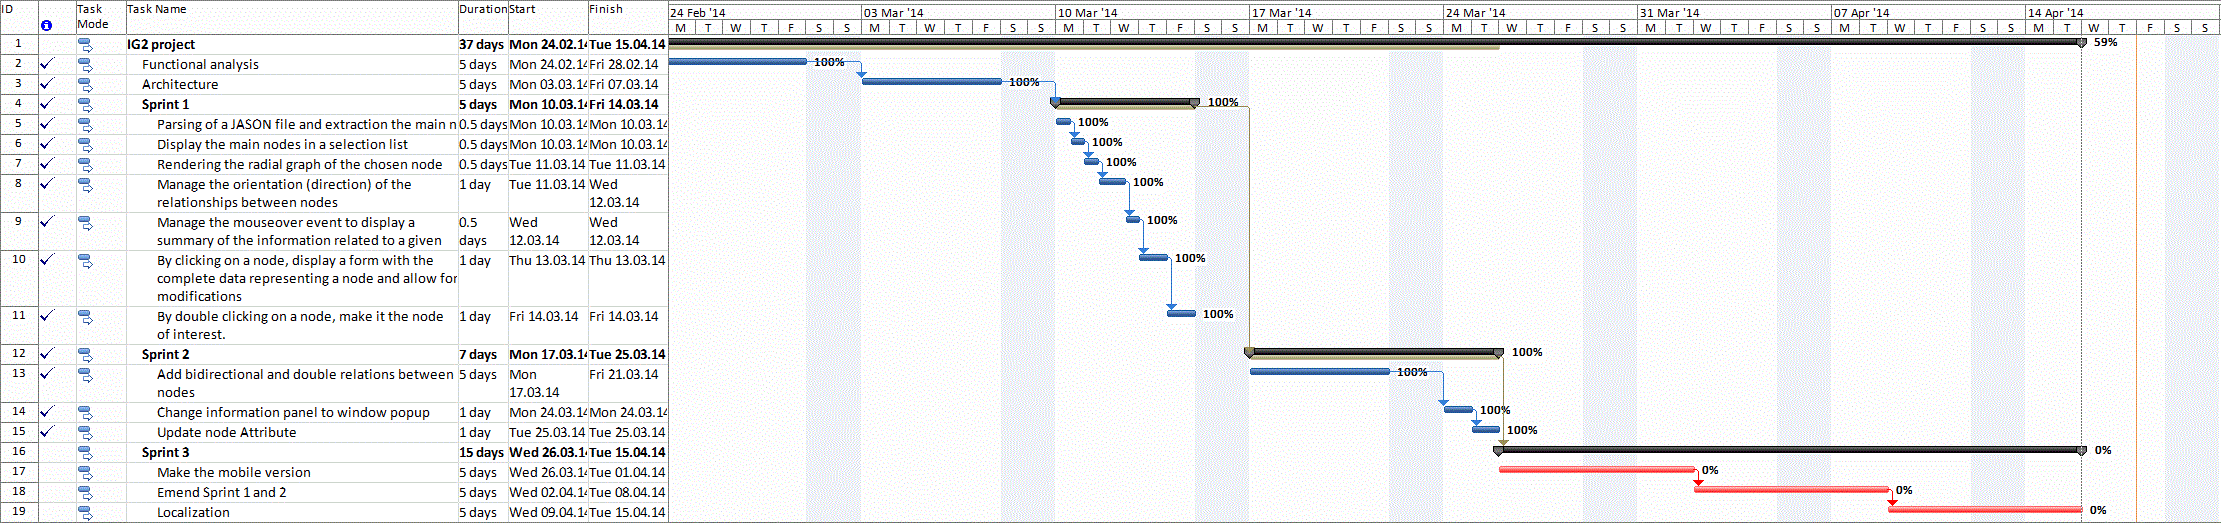
\includegraphics[scale=0.3, frame]{IG2_Manel_A.png}
\caption{The $IG�$ project plan}
\end{figure}
\vspace*{\fill}
\end{landscape}
\end{center}
\newpage
\begin{figure}[h]
\centering
\includegraphics[width=\hsize , frame]{IG2_P1.png}
\caption{List of scheduled tasks}
\end{figure}

%\newpage
%\begin{figure}[!h]
%\centering
%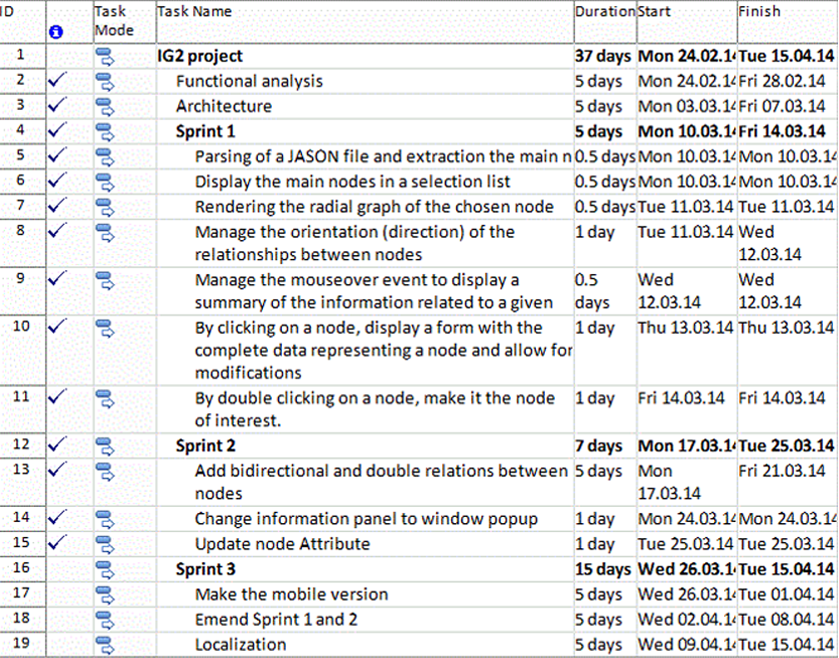
\includegraphics[scale=0.3]{IG2_P11.png}
%\caption{Schedule Sprint}
%\end{figure}
%
%\begin{figure}[!h]
%\centering
%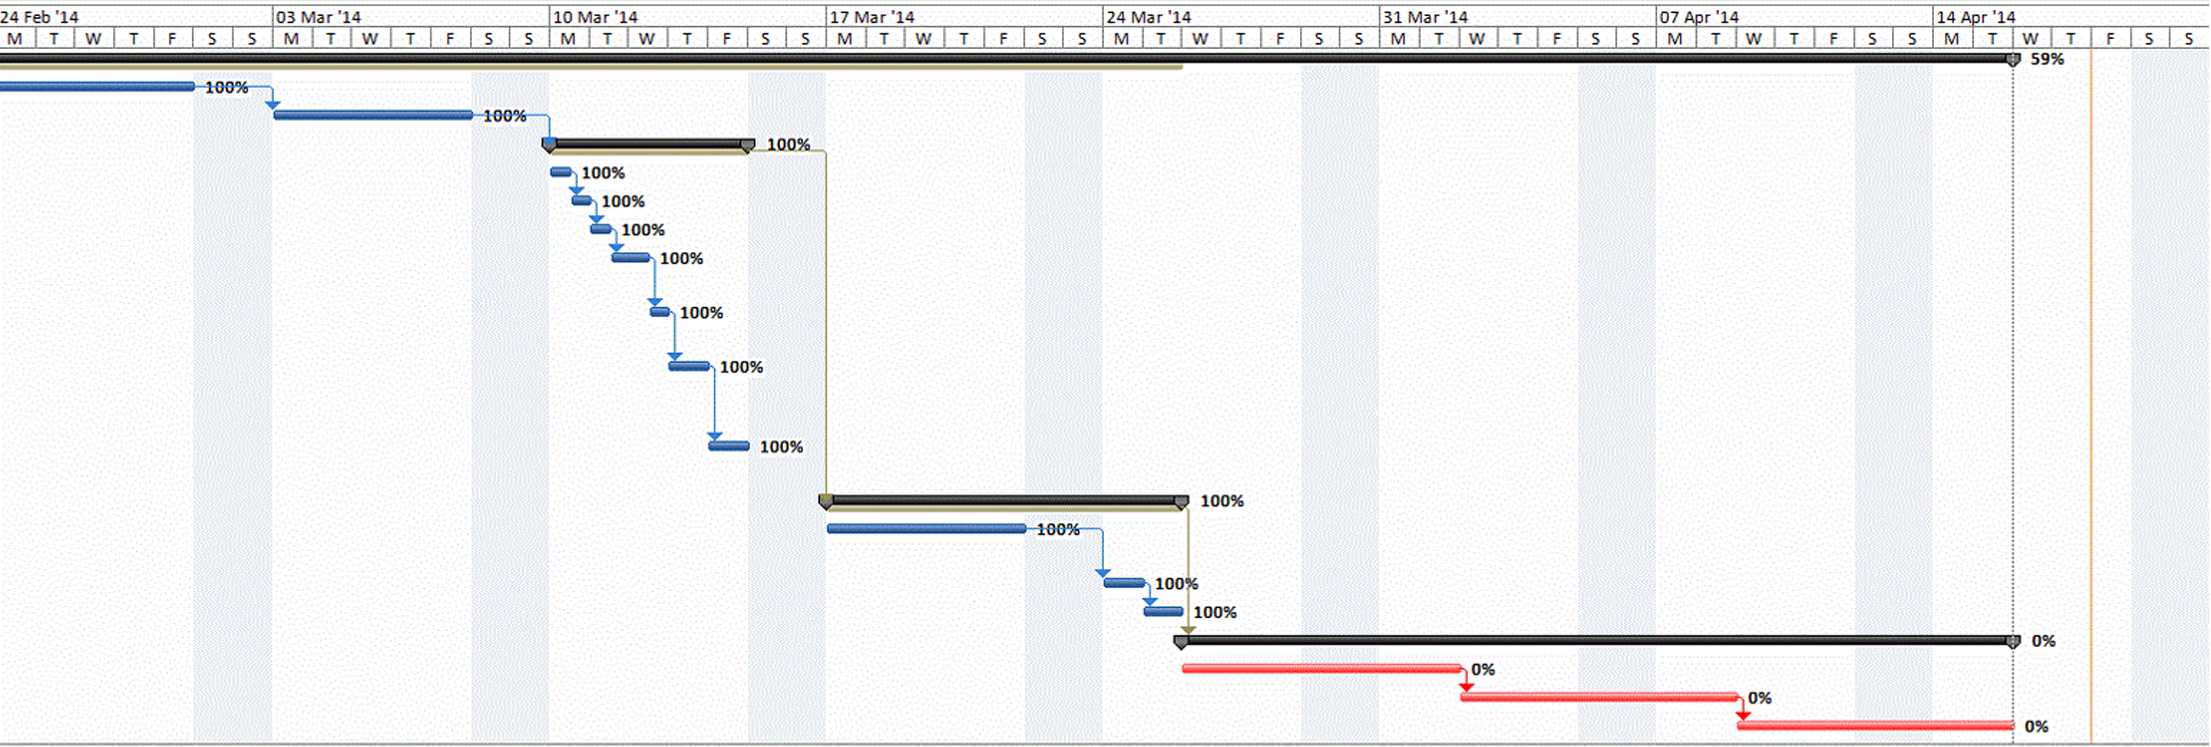
\includegraphics[scale=0.2]{IG2_P22.png}
%\caption{GANTT diagram}
%\end{figure}
\paragraph*{}
The project in its current state was achieved in three sprints. In the first sprint the development environment has been prepared, and a prototype allowing to parse a JSON file and to visualize a radial graph was developed. More details can be found the (paragraph of the 1st sprint). In the second sprint we mainly focused on the management of the nodes and the relations. The update node/relation was a significant part of this sprint.
While developing the second sprint of the project I suggested to the team to localize the user interface. The $IG�$ application is dedicated to an international market and it is very important to allow different people to use it in their mother tongue. Stradfi SA team has appreciated the idea and has expressed its interest to realize this feature in the 3rd sprint.
\section{The overall list requirements}
\paragraph*{}
The product backlog represents the list of the requirements to implement. At the beginning of the project, not all of the requirements are known. Thus some modifications may occur by adding and/or removing some requirements. However, the product owner is asked to prioritize the mastered requirements in order to prepare each sprint's backlog. The following table presents the detailed product backlog in its final form as discussed with team.
\begin{table}[h]
\begin{tabular}{|p{15cm}|}
\hline
\textbf{List} \\
\hline
1.Kick-off meeting \\
\hline
2. Server configuration  \\
\hline
3. Creating oh th JSON files  \\
\hline
4. Architecture and methodology approval \\
\hline
5. Parsing of JSON file \\
\hline
6. Listing of the available objects \\
\hline
7. Rendering the Radial Graph of the selected object \\
\hline
8. Managing the orientation (direction) of the relationships between nodes \\
\hline
9. Implementation of the mouseover event to display a summary of the information related to a given node \\
\hline
10. Accessing to a node attributes and properties \\
\hline
11. Selection of the node of interest \\
\hline
12. Implementation of different types of relations \\
\hline
13. Implementing the features allowing to update the properties and attributes of a given node \\
\hline
14. Implementation the support of different languages \\
\hline
15. Implementing the zoom in and zoom out feature \\
\hline
16. Implementing Drag and Drop capablity \\
\hline
17. Implementing the responsivity \\
\hline
17. Implementing the mouseover support for edges \\
\hline
19. Manage Dropdown list for Type, Aspect and Salutation attribute \\
\hline
\end{tabular}
\caption{The list of Requirements}
\end{table}
\paragraph*{}
The list of requirements shown above has been organized, prioritized and implemented in four sprints. The details of each of them is presented in the next chapter. 
\section{Conclusion}
\paragraph*{}
The kick-off meeting was really very helpful for the project initiation. It clarified things that are very important to achieve a project such as the methodology to adopt and product backlog. This gives the departure signal for the development that has been also done according to the different sprints described above. The overall project plan was also defined during the kick-off meeting and approved during the sprint "zero". The detailed aspects of the implementation are discussed in the next chapter.
\renewcommand{\thepage}{}
\chapter{Realization}
\thispagestyle{empty}
\pagestyle{fancy}
\lhead{\small \bf  Chapitre 5: Realization}
\rhead{}
\chead{}
\renewcommand\thepage{\arabic{page}}
 \setcounter{minitocdepth}{1}
\minitoc
\clearpage
\section{Introduction}
\lettrine[lines=2,lhang=0.44,lraise=0,loversize=0.08,findent=-0.11em,slope=0.6em]%
{T}{} he $ IG� $ application is Web oriented. The analysis of the initial specifications has lead us to distinguish three different layers: 
\begin{itemize}
\item The UI interface allowing users to interact with the application (selecting objects and nodes, displaying graphs, etc.)
\item The logic that explores and organizes the data.
\item The data layer that contains the information specifying objects and entities.
\end{itemize}
\paragraph*{}
It is therefore obvious to adopt a 3-tiers architecture to implement the application: the presentation tier (the UI), the business tier (the logic layer) and the data layer. The implementation of the application was also based on the Model-View-Controller (MVC) [W12] paradigm. Using WEB 2.0 and MVC easily fit with the 3-tiers architecture and the needs expressed by Stradefi SA.
\section{The MVC Architecture}
\paragraph*{}
MVC [7][W12] - Model-View-Controller - is a design pattern for the architecture of Web applications.
\begin{figure}[h]
\centering
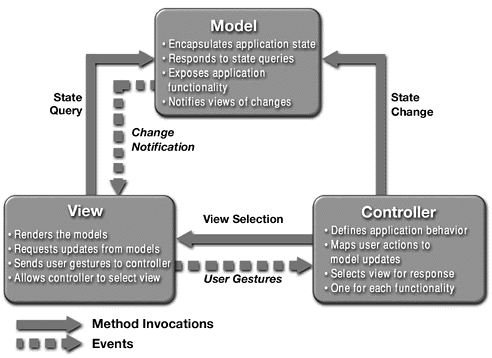
\includegraphics[scale=0.8]{mvc.png}
\caption{MVC model}
\end{figure}
\paragraph*{}
It is a widely adopted pattern, across many languages and implementation frameworks, whose purpose is to achieve a clean separation between three components of most any Web application:
\begin{itemize}
\item Model: business logic & processing
\item View: user interface (UI)
\item Controller: navigation & input
\end{itemize}
\paragraph*{}
MVC benefits fall into multiple categories:
\begin{itemize}
\item Separation of concerns in the codebase
\item Developer specialization and focus
\item Parallel development by separate teams
\end{itemize}
\paragraph*{}
In looking at these in a little more detail, it will become clear that the second two bullet-points are corollaries of the first.
\section{The 3-tiers architecture point of view of the $ IG� $}
\paragraph*{}
The development was based on HTML5, CSS3 and JavaScript. The presentation layer is based on these languages and technologies. The JIT library (�II.2.1), developed in JavaScript, combined with HTML allowed implementing easily the UI.
\paragraph*{}
The data layer, in the current state of the development uses only JSON files, however the application is open enough to support XML (using a DOM parser) or any other of structured data format (databases for instance).
\paragraph*{}
At the present time there's no clear separation between the business layer and the presentation layer. Indeed, we use the JIT native parser to parse JSON files and to render the corresponding radial graphs. As mentioned in the perspectives (� FUTUR), a very important part of the logic is not yet implemented and needs extra developments that do not depend on the JIT library.
\section{The MVC architecture point of view of the $IG�$}
\paragraph*{}
The model represents the underlying logical structure of the data used by the application (JSON files). This data model doesn't contain any information about the user interface and could therefore be used with other views and/or controllers.
\paragraph*{}
The view is the user interface itself. The view depends on the used device and adapts to the hardware constraints. The view cannot be reused except with compatible devices.
\paragraph*{}
The controller represents the way to communicate between the data model and the view. In the $IG�$ application two controllers have been taken into account: the first one allows the usage of a keyboard and mouse and the second one, which is suitable for mobile devices, allows the usage of the touch-pad and touch-screen.
\section{The logical architecture}
\paragraph*{}
The software components used by the application have been identified through the whole process of analysis and specification that has been conducted before the beginning of the development. The Web nature of the applications imposes the usage of an application server. The visualization of the radial graphs requires the usage of a rendering engine. despite the structured nature of the data used by the application, we made the choice not to consider a data base but rather use text files (JSON) that are natively supported by JavaScript. The overall logical architecture of the $IG�$ application is presented in the figure V.2.
\begin{figure}[h]
\centering
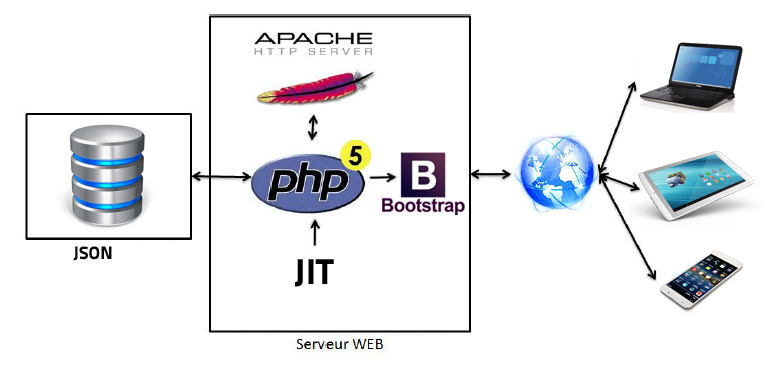
\includegraphics[scale=0.5, frame]{architechturesysteme.png}
\caption{Logical architecture}
\end{figure}
\paragraph*{}
The rendering engine is the JIT library (�II.2.1). The other software modules used for the development and the deployment of the application are: Apache HTTP server, PHP and Bootstrap.
\begin{itemize}
\item \textbf{Bootstrap:} Bootstrap[W13] is a free collection of tools for creating websites and web applications. It contains HTML and CSS-based design templates for typography, forms, buttons, navigation and other interface components, as well as optional JavaScript extensions. It is the No.1 project on GitHub with 65,000+ stars and 23,800 forks (as of March 2014) and has been used by NASA and MSNBC, among many others.
\item \textbf{PHP5:}PHP [W14] is a server-side scripting language designed for Web development but also used as a general-purpose programming language. As of January 2013, PHP was installed on more than 240 million websites (39\% of those sampled) and 2.1 million Web servers. Originally created by Rasmus Lerdorf in 1995, the reference implementation of PHP is now produced by The PHP Group. While PHP originally stood for Personal Home Page, it now stands for PHP: Hypertext Preprocessor, a recursive backronym.
PHP code can be simply mixed with HTML code, or it can be used in combination with various templating engines and Web frameworks. PHP code is usually processed by a PHP interpreter, which is usually implemented as a Web server's native module or a Common Gateway Interface (CGI) executable. After the PHP code is interpreted and executed, the Web server sends resulting output to its client in form of a generated Web page. PHP has also evolved to include a command-line interface (CLI) capability and can be used in standalone graphical applications.
PHP is free software released under the PHP License. PHP has been widely ported and can be deployed on most Web servers on almost every operating system and platform, free of charge.
\item \textbf{Apache HTTP Server} is a Web server application, it's a HTTP server created and maintained whitin the Apache foundation {\color[rgb]{0.41,0.41,0.41}\href{httpd.apache.org}{\textbf{10}}}. It's the most HTTP server popular on the World Wide Web {\color[rgb]{0.41,0.41,0.41}\href{http://webfoundation.org/}{\textbf{11}}}.
\end{itemize}
The Data layer is represented by various \textbf{Json}{\color[rgb]{0.41,0.41,0.41}\href{http://www.json.org/}{\textbf{8}}} files. 
\section{Class diagram}
\paragraph*{}
The design of the $IG�$ application provided us with the following class diagram (Figure V.3). Although the resulting implementation of $IG�$ is not object oriented, the class diagram helped us organizing the data layer, especially the structure of JSON files. We also used the OOTB features of JIT to implement the user interface.
\newpage
\begin{figure}[h]
\begin{center}
\includegraphics[scale=0.6, frame]{ClassDiagram.png}
\end{center}
\caption{$IG�$ Class Diagram}
\end{figure} 
\section{The sprints' achievement}
\paragraph*{}
Among all the requirements that have been defined in the $ IG� $ specifications, the most significant ones have been considered and defined as the product backlog. All of the considered requirements have been prioritized and organized as sprints. Actually four sprints has been achieved: "the project initiation sprints" (aka sprint "zero"), "the graph rendering sprint" (aka sprint "one"), "updating nodes' properties and managing relations sprint" (aka sprint "two") and the "localization sprint" (aka sprint "three").
\subsection{Sprint "zero": Project initiation}
\paragraph*{}
The project started by the analysis of the specifications given by Stradefi SA. Some conference calls have been done with Stradefi SA Office at Geneva to define the different roles of the team members and to identify the product backlog. A kick off meeting has also been done and officially started the project. The project plan was achieved in this sprint.
\begin{table}[h]
\begin{center}
\begin{tabular}{|p{7cm}|p{3cm}|p{3cm}|}
\hline
\multicolumn{3}{|c|}{Sprint "zero": Project initiation}  \\
\hline
\textbf{Tasks} & \textbf{Deadline} & \textbf{Date }\\
\hline
Kick-off meeting& 2 hours &  9 March \\
\hline
Server configuration & 3 Hours & 9 March \\
\hline
Architecture and methodology approval & 1 day & 9 March \\
\hline
\end{tabular}
\end{center}
\caption{Backlog product - Sprint "zero"}
\label{Backlog product - Sprint "zero"}
\end{table}
\subsection{Sprint "one": Rendering a radial graph}
\paragraph*{}
The development has really started during this sprint. We first focused on the parsing of JSON files, the identification of what could be represented as a node and what will play the role of a relation. Finally, the data extracted from the JSON files is given to the rendering engine in order to deal with it and to display the radial graph. The following table presents the sprint "one" backlog.
\begin{table}[h]
\begin{center}
\begin{tabular}{|p{7cm}|p{3cm}|p{3cm}|}
\hline
\multicolumn{3}{|c|}{Sprint "one": Rendering a radial graph}  \\
\hline
\textbf{Tasks} & \textbf{Deadline} & \textbf{Date }\\
\hline
Parsing of JSON file & 3 hours week & \multirow{7}{*}{27 March}  \\
\hline
Listing of the available objects & 4 hours & 27 March \\
\hline
Rendering the Radial Graph of the selected object & 3 hours & 27 March   \\
\hline
Managing the orientation (direction) of the relationships between nodes & 1 day & 27 March\\
\hline
Implementation of the mouseover event to display a summary of the information related to a given node & 3 hours & 27 March \\
\hline
Accessing to a node attributes and properties & 1 day & 27 March \\
\hline
Selection of the node of interest & 1 day & 27 March \\
\hline
\end{tabular}
\end{center}
\caption{Backlog product - Sprint "one"}
\label{Backlog product - Sprint "one"}
\end{table}
\subsubsection{Detailed design of Sprint "one"}
\paragraph*{}
The Figure V.4 presents the detailed design of sprint "one", its design the actions and events released, the user can use it to navigate on the application. 
\newpage
\begin{figure}[h]
\centering
\includegraphics[scale=0.7, frame]{renderingDiagram.png}
\caption{Rendering a radial graph Sequence Diagram}
\end{figure}
\subsubsection{Implementation and execution of Sprint "one"}
\paragraph*{}
When the user logs in, the first screen of the user interface the list of available objects, that he can access to (Figure V.5). The user can select an object in order to display the corresponding graph. 
\newpage
\begin{figure}[h]
\begin{center}
\includegraphics[scale=0.6, frame]{visualizeGraph.png}
\end{center}
\caption{The list of available objects}
\end{figure}
\paragraph*{}
When the user selects an object, the corresponding radial graph is displayed. The node corresponding to the object first selected by the user becomes the node of interest (Figure V.6).
\begin{figure}[h]
\centering
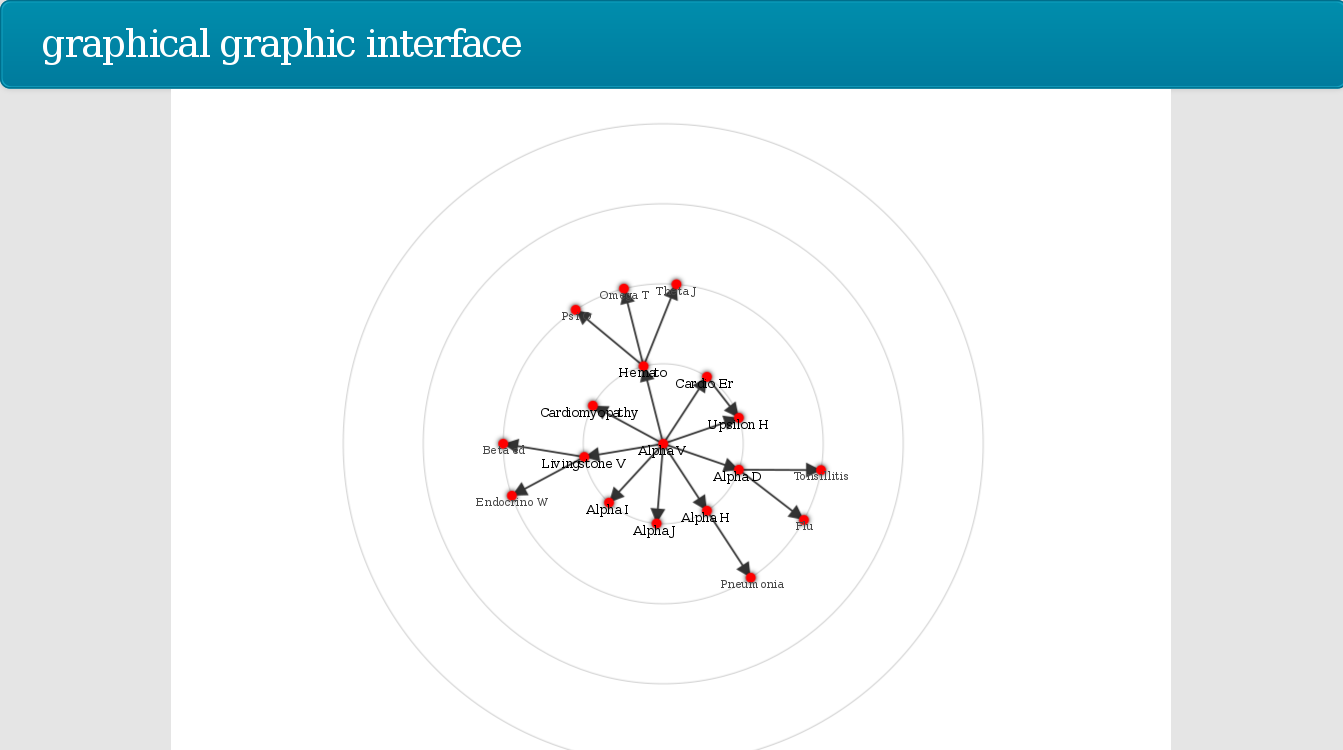
\includegraphics[scale=0.3, frame]{InterfaceGraph.png}
\caption{Node of the interest and its properties}
\end{figure}
\paragraph*{}
The user can change the node of interest by clicking on the label of the node. When the user click on the label of the node, a label appear contains the properties of the node of interest (Figure V.7).
\begin{figure}[h]
\centering
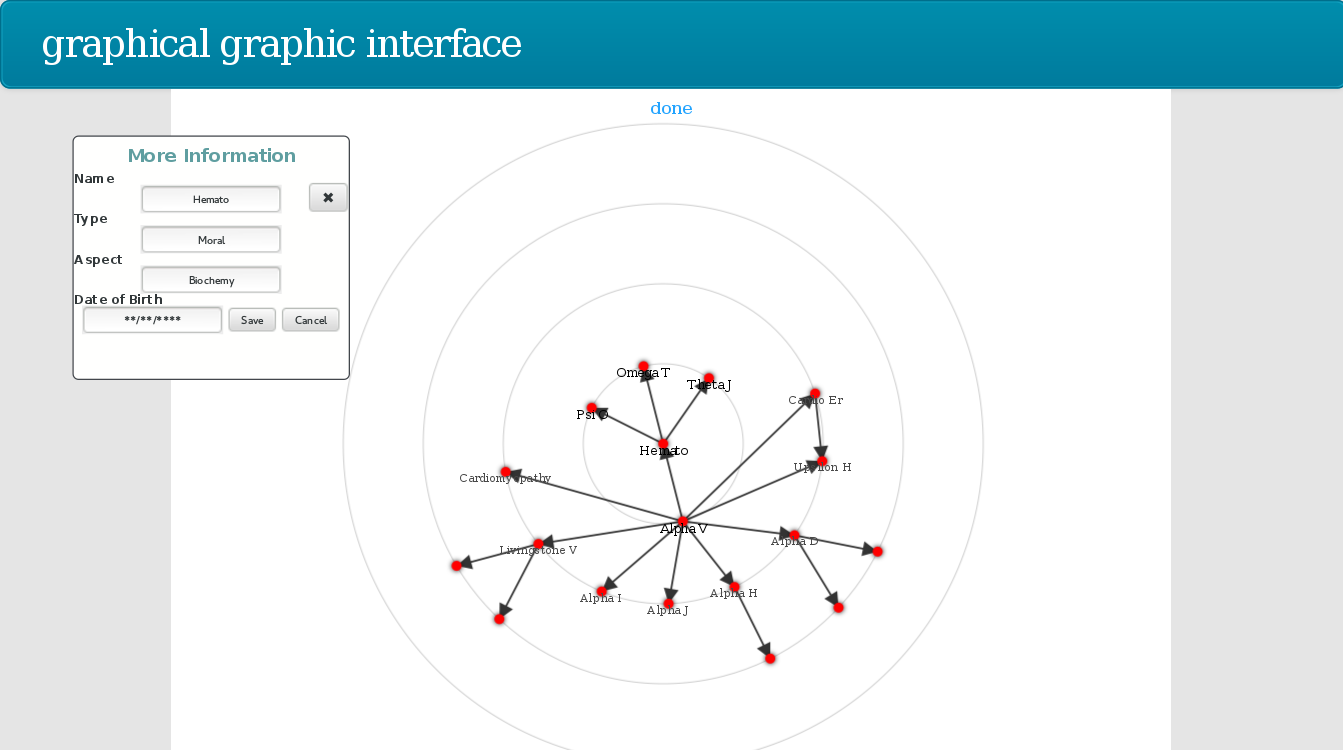
\includegraphics[scale=0.3, frame]{centericnode.png}
\caption{Interest node with her informations}
\end{figure}
\subsection{Sprint "two": managing relations and updating the nodes properties}
\paragraph*{}
In the sprint "one", only the unilateral relations have been taken into account. However, the $ IG� $ application requires relations to be unilateral, bilateral or multiple. In this sprint we implemented all the types of relations required in the specification.
We also developed a feature allowing to access to a given node properties and to add, remove or update any property.
\begin{table}[h]
\begin{center}
\begin{tabular}{|p{7cm}|p{3cm}|p{3cm}|}
\hline
\multicolumn{3}{|c|}{Sprint "two": managing relations and updating the nodes properties }  \\
\hline
\textbf{Tasks} & \textbf{Deadline} & \textbf{Date }\\
\hline
Implementation of different types of relations & 2 days & 25 April\\
\hline
Change information panel to pop-up window & 1 day & 25 April \\
\hline
Implementing the features allowing to update the properties and attributes of a given
node & 2 days & 25 April \\
\hline
\end{tabular}
\end{center}
\caption{Backlog product - Sprint "two"}
\label{Backlog product - Sprint "two"}
\end{table}
\subsubsection{Detailed design of sprint "two"}
\paragraph*{}
The Figure V.8 shows the detailed design to update node properties
\newpage
\begin{figure}[h]
\begin{center}
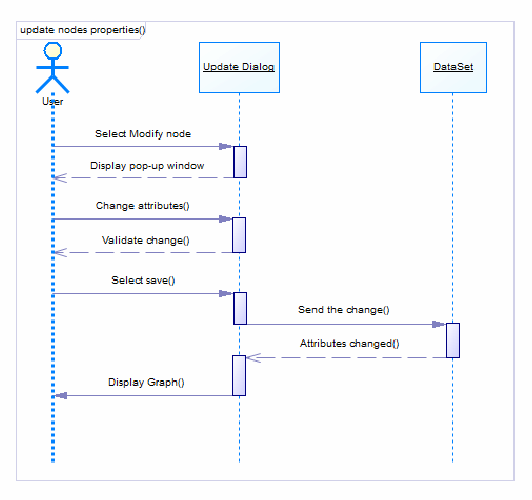
\includegraphics[scale=0.7, frame]{UpdateSEC.png}
\end{center}
\caption{Update the node properties Sequence Diagram}
\end{figure}
\subsubsection{Implementation and execution of Sprint "two"}
\paragraph*{}
The Figure V.9 presents the different types of relations. The type 1 represents unilateral/simple relation, type 2 is bilateral relation and of type 3 is multiple relation. 
\newpage
\begin{figure}[h]
\centering
\includegraphics[scale=0.4, frame]{types-of-relations.png}
\caption{types a relations handled by $IG�$}
\end{figure}
\paragraph*{}
The Figure V.10 presents the dialog, allowing users to update a given node properties.
\begin{figure}[h]
\centering
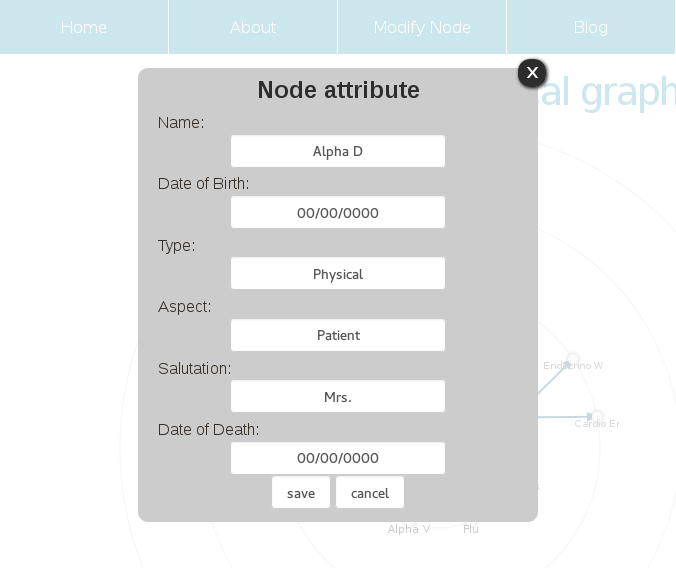
\includegraphics[scale=0.4, frame]{popupwin.png}
\caption{Updating a node}
\end{figure}
\subsection{Sprint "three": $IG�$ localization}
\paragraph*{}
The localization wasn't a requirement expressed in the specifications. During a discussion with the product owner, I noticed that the $IG�$ audience is international and I suggested to also consider the localization of the user interface in the development. The team has approved my suggestion and asked me to implement this feature in this sprint.
\begin{table}[h]
\begin{center}
\begin{tabular}{|p{7cm}|p{3cm}|p{3cm}|}
\hline
\multicolumn{3}{|c|}{Sprint3: Multilanguage and maanaging the Web application version}  \\
\hline
\textbf{Task} & \textbf{Deadline} & \textbf{Date }\\
\hline
Implementation the support of different languages & 3 days & 3 May \\
\hline
Implementing the zoom in and zoom out feature & 3 Hours & 3 May \\
\hline
Implementing Drag and Drop capablity & 3 hours & 3 May \\
\hline
Implementing the responsivity  & 2 Days & 3 May   \\
\hline
Implementing the mouseover support for edges & 2 days & 3 May\\
\hline
Manage Dropdown list for Type, Aspect and Salutation attribute & 1 hours & 3 May\\
\hline
\end{tabular}
\end{center}
\caption{Product Backlog - Sprint "three"}
\label{Product Backlog - Sprint "three"}
\end{table}
\subsubsection{Implementation and execution of Sprint "three"}
\paragraph*{}
As already mentioned  �V.7.4 the $IG�$ application is intended to be used by a wide international audience. The implementation of the software has been done in such a way that it allows the support of various locales. The user  interface language is therefore configurable. We have experimented  $IG�$ with Latin languages (French,English,Spanish,etc.), Arabic and Chinese. The Figure V.11 is a screen-shot of the English user interface of $IG�$. The Figure V.12 presents the Arabic user interface and the Chinese one is presented in the Figure  V.13
\begin{figure}[h]
\centering
\includegraphics[scale=0.4, frame]{en-lang.png}
\caption{French interface}
\end{figure}
\newpage
\paragraph*{}
\begin{figure}[h]
\centering
\includegraphics[scale=0.4, frame]{ar_lang.png}
\caption{Arabic interface}
\end{figure}
\newpage
\begin{figure}[h]
\centering
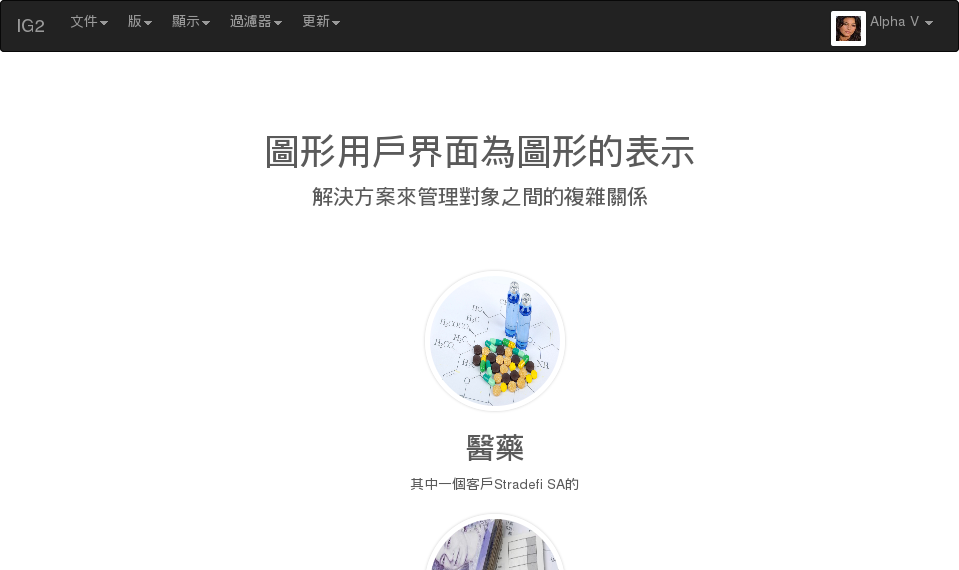
\includegraphics[scale=0.4, frame]{ch-lan.png}
\caption{Chinese interface}
\end{figure}
\paragraph*{}
The Chinese translation was done, thanks to google translator (https://translate.google.com) this translation is therefore approximate and may contain some mistakes.
\chapter*{Conclusion}
\phantomsection
%\addcontentsline{toc}{chapter}{General Conclusion}
\addstarredchapter{General Conclusion}
 \pagestyle{fancy}
 \thispagestyle{\renewcommand{\headrulewidth}{0pt}}
\rhead{}
\lhead{}
\lettrine[lines=2,lhang=0.44,lraise=0,loversize=0.08,findent=-0.11em,slope=0.6em]%
{A}{} proverb is a simple and concrete saying popularly known and revered, which expresses a truth, based on common sense or the practical experience of humanity. The proverb "A picture is worth 1000 words" is one you have probably heard more than once.
\paragraph*{}
Informed decision making is the foundation upon which successful businesses are built. As a decision maker, one needs access to highly visual business intelligence tools that can help making the right decisions quickly. As organizations grow, so does the amount of collected information. If this data is delivered in spreadsheets or tabular reports, it becomes more and more challenging to find the patterns, trends and correlations necessary to well perform the required job.
\paragraph*{}
The practice of representing information visually is nothing new. Scientists, students, and analysts have been using data visualization for centuries to track everything from astrological phenomena to stock prices. Only recently, with the adoption of more sophisticated BI technology in the corporate world and the ever-increasing practice of data collection and data mining activities, has data visualization in the form of dashboards been used as an important presentation tool in business analysis. As a result, the use of dashboards in making quick and accurate business decisions has become an essential requirement for remaining competitive. The common forms of data visualization are Basic Charts and Status Indicators. This remains very useful however the nature of data managed by the organizations has evolved and became more and more complex. More advanced data visualizations forms were needed. This includes scatter graphs, bubble charts, spark line charts, geographical maps, tree maps, Pareto charts, and many others. These more sophisticated visualizations are designed to display data in ways tailored to a specific function or industry.
\paragraph*{}
Decision makers need to interact with their data to expose trends, highlight opportunities and raise red flags quickly and accurately. Their data should answer key questions and provide insight into issues that contribute directly to the decision making process. Presenting this data visually and adding contextual information to complement the analysis process not only makes it quicker and easier to pinpoint areas of opportunities and concern, but also enables decision makers to take action with their data. Successful data visualization provides the ability to expose problem areas and communicate those problems universally. Not being able to clearly identify and share your discoveries to back up your decisions can mean the difference between taking appropriate and decisive action and losing momentum or failing to act.
\paragraph*{}
Using data visualization to display large amounts of data is nothing new. However, its value and use in making business decisions is often overlooked or poorly implemented. The key to success in using data visualization is ensuring that: the best and most appropriate types of visualizations are used; the data is always put into perspective with contextual information allowing for the information to be universally understood; and that the data being measured within the data visualization enables the user to take action based on the observations being made. With a good set of visuals that keep these key success factors in mind, decisions can be made more quickly and with more confidence so that your business can continue to grow.
\paragraph*{}
It is in this exciting and intellectually challenging and motivating setting that I did my internship graduation. The past months have been very instructive for me. Stradefi SA has offered me opportunities to learn and develop myself in many areas. I gained a lot of experience, especially in the Data Visualization field as well as the project planning and monitoring. I also developed my skills in the design and programming of significant software solutions. A lot of the tasks and activities that I have worked on during my internship are familiar with what I?m studying at the moment. I worked in many areas where I did different work.
I also learned what working in a team really means. The sense of the term "Deadlines" has another dimension in my mind. I acquired a the meaning of the "rigorous work", things they would not teach me of in college: only confrontation with the reality of work allows us to understand and grow. 
%============ Bibliographie ============%
\renewcommand{\bibname}{Bibliography}
\lhead{}
\addcontentsline{toc}{chapter}{Bibliography}
\begin{thebibliography}{20}
\bibitem[1]{1} Graph Theory, Rienhard Diestel, Spriner Verlag, Heidelberg - 2005
\bibitem[2]{2} Graph Theroy, Keijo Ruohonen, Lecture notes in Graph Theory, Tampere University of Technology, Finland.
\bibitem[3]{3}	Radial Edge Splatting for Visualizing Dynamic Directed Graphs; Michael Burch, Fabian Beck and Daniel Weiskopf. In proceeding of the International Joint Conference on Computer Vision, Imaging and Computer Graphics Theory and Applications, 24 - 26 February 2012 - Rome, Italy.
\bibitem[4]{4} Radial Tree Graph Drawing Algorithm for Representing Large Hierarchies; Greg Book & Neeta Keshary, internal report of the University of Connecticut, December 2001
\bibitem[5]{5} Optimizing a radial layout of bipartite graphs for a tool visualizing security alerts; Maxime Dumas, Michael J. McGu?n, Jean-Marc Robert and Marie-Claire Willig. Lecture Notes in Computer Science Volume 7034, 2012, pp 203-214
\bibitem[6]{6} Data Processing and Visualization Tools; European Public Sector Information Platform, Topic Report No. 2013/07 
\bibitem [7]{7}D3 Tips and Tricks, Interactive Data Visualization in a Web Browser; Malcolm Maclean, Lean Publishing, 2013.
\bibitem[8]{8} JavaScript (HTML5, CSS3) Toolkits for InfoVis (Graphics); Amir Kanuric, Raoul Rubien, Jorg Schlager, Graz University of Technology, Survey on JavaScript InfoVis tools.
\bibitem[9]{9} Development of InfoVis Software for Digital Forensics; Grant Osborne, Benjamin Turnbull and Jill Slay. 2012 IEEE 36th International Conference on Computer Software and Applications Workshops, pp 213-217.
\bibitem[10]{10} M. Poppendieck, "A History of Lean: From Manufacturing to Software Development," in JAOO Conference, Aarhus, Denmark, 2005.
\bibitem[11]{11} J. K. Liker, The Toyota way: 14 Management Principles from the World's Greatest Manufacturer. New York: McGraw-Hill, 2004.
\bibitem[12]{12} W. D. Holford and M. Ebrahimi, "Honda: Approach to Innovation in Aerospace and Automotive/Pick-Up Truck Development: A Dialectical Yet Coherent Firm," in 40th Annual Hawaii International Conference on System Sciences (HICSS-40), Big Island, Hawaii, 2007.
\bibitem[13]{13} H. Takeuchi and I. Nonaka, Hitotsubashi on Knowledge Management. Singapore: John Wiley & Sons (Asia), 2004.
\bibitem[14]{14} P. M. Senge, The Fifth Discipline: the Art and Practice of the Learning Organization. New York: Currency, 1990.
\bibitem[15]{15} K. Schwaber, Agile project management with Scrum. Redmond, Wash.: Microsoft Press, 2004.
\bibitem[16]{16} K. Schwaber and M. Beedle, Agile software development with scrum: Prentice Hall, 2002.
\end{thebibliography}

\clearpage
%============ Bibliographie ============%
\renewcommand{\bibname}{Webography}
\lhead{}
\addcontentsline{toc}{chapter}{Webography}
\begin{thebibliography}{20}
\bibitem[W1]{W1} [\url{http://en.wikipedia.org/wiki/Radial\_ tree}]; last visit 17 April 2014; last modified on 9 May 2014.
\bibitem[W2]{W2} [\url{http://en.wikipedia.org/wiki/Force-based\_ layout}]; last visit on 17 April 2014; last modification on 16 January 2014.
\bibitem[W3]{W3}[\url{http://en.wikipedia.org/wiki/Directed\_ graph}]; last consult 17 April 2014; Modified 3 April 2014.
\bibitem[W4]{W4} [\url{http://d3js.org/}];last visit 17 April 2014
\bibitem[W5]{W5} [\url{http://philogb.github.io/jit/}];last visit 17 April 2014
\bibitem[W6]{W6} [\url{http://sigmajs.org/}]; last visit 17 April 2014.
\bibitem[W7]{W7} [\url{http://www.senchalabs.org/}]; last visit 17 April 2014.
\bibitem[W8]{W8} [\url{http://en.wikipedia.org/wiki/Waterfall\_ model}]; last visit 17 April 2014; last modification 3 May 2014.
\bibitem[W9]{W9} [\url{http://en.wikipedia.org/wiki/V-Model\_\%\ 28software\_ development\%\ 29}] V-Model software developement From Wikipedia; last visit 17 April 2014; last modification 1 April 2014.
\bibitem[W10]{W10} [\url{http://en.wikipedia.org/wiki/Iterative\_ and\_ incremental\_ development}] Incremental software developement, From Wikipedia; last visit 17 April 2014; last modification 14 May 2014.
\bibitem[W11]{W11} [\url{http://en.wikipedia.org/wiki/Scrum\_ \% 28software\_ development\% 29}] Scrum software developement; From Wikipedia; last visit 17 April 2014; last modification 18 May 2014.
\bibitem[W12]{W12} [\url{https://ist.berkeley.edu/as-ag/pub/pdf/mvc-seminar.pdf}] Model-View-Controller: A Design Pattern for Software. Presented in a seminar of Berkley University in 2004. 
\bibitem[W13]{W13} [\url{http://en.wikipedia.org/wiki/Bootstrap\_\% 28front-end_framework\%29}] Bootstrap (front-end framework) From Wikipedia, the free encyclopedia; 
\bibitem[W14]{W14} [\url{http://en.wikipedia.org/wiki/PHP}] PHP From Wikipedia, the free encyclopedia 
\bibitem[W15] {W15} [\url{http://philogb.github.io/blog/2008/05/07/rgraph-quick-tutorial/}] Feeding JSON tree structures to the JIT;Posted in: javascript infovis toolkit 
\bibitem[W16]{W16} [\url{http://philogb.github.io/blog/2008/04/27/on-controllers/}] On controllers; Posted in: javascript infovis toolkit 
\bibitem[W17]{W17} [\url{http://philogb.github.io/jit/static/v20/Docs/files/Core/Core-js.html}]; JavaScript InfoVis Toolkit Documentation 
\end{thebibliography}
\clearpage
\appendix
%\chapter{Annexe A: Numbty}
\paragraph*{}
\textbf{Numbty:} a numbty is a person whose brain is totally numb. In this context, numb means "deprived of feeling or the power of unassisted activity"; in general, a numbty needs the stimulation of an electric cattle prod to even get to the right office in the morning. Communication with numbties is severely hampered by the fact that although they think they know what they mean (which they do not), they seldom actually say it, and they never write it down. And the main employment of numbties world-wide is in creating project specifications. You must know this - and protect your team accordingly.
%\chapter{Annexe B: Radial exampl}
\paragraph*{}
This example shows:
\begin{itemize}[font=\color{black}, label=\maltese]
\item A radial graph
\item The selected node is "S", as "X" is a direct linked node (level 1), Y a level 2 linked node and F
must not be depicted in the picture because it is not linked to a level 1, F is a level 3 node
\item Relations with arrows, unidirectional "in" and unidirectional "out" and bidirectional
\end{itemize}
\begin{figure}[h]
\centering
\includegraphics[scale=0.5, frame]{RadialGraph.png}
\caption{Radial Graph}
\end{figure}
\newpage
\textbf{Radial}
The chosen node is the center of the graph\\
The linked nodes are organized on circles (aka orbit) as per distance level\\
Rules: when a node "A" is linked with two (or more) nodes of situated on different orbits, the node is
placed on the lowest orbit as possible. For example:
\begin{itemize}
\item Node$_$ a is the central node
\item Node$_$ a is linked with Node$_$ b and node$_$ c \rightarrow Node_b and Node_c are on orbit 1
\item If Node$_$b and Node$_$ c are linked it creates a transversal relation of the same level
\item Node$_$ b is linked with Node$_$ d \rightarrow node$_$ d is on orbit 2
\item Node$_ $c is linked with Node$_$ e \rightarrow node$_$ e is on orbit 2
\item Node$_$ e is linked with Node$_$ f \rightarrow node$_$ f is on orbit 3 at this point, when continuing the exploration we notice that:
\begin{itemize}
\item Node$_$ f is linked with Node$_$b \rightarrow node$_$ f is promoted to orbit 2 Please note that the
exploration does not take into account the link direction property, that can make the
exploration more recursive.
\end{itemize}
\end{itemize}
\paragraph*{}
Biradial and triradial might be an option to be developed in a later stage if useful. A biradial will consist in selecting two nodes and a triradial three nodes. These nodes might not have a common a common link. The selected nodes must be displayed on the screen harmoniously (in triangle for a triradial graph). This feature might be required to show how two or threee nodes are linked together
%\chapter{Annexe C: Parsing JSON tree structure to the JIT}
\paragraph*{}
The tree structure that feeds the spacetree, hypertree, treemap and rgraph visualizations[W15] is always the same. Roughly speaking, the JSON tree structure consists of tree nodes, each having as properties:
\begin{itemize}
\item id a unique identifier for the node.
\item name a node's name.
\item data The data property contains a dataset. That is, an array of key-value objects defined by the user.
\end{itemize}
\paragraph*{}
Roughly speaking, this is where you can put some extra information about your node. You'll be able to access this information at different stages of the computation of the JIT visualizations by using a controller.
children An array of children nodes, or an empty array if the node is a leaf node. For example:
\begin{center}
\begin{figure}
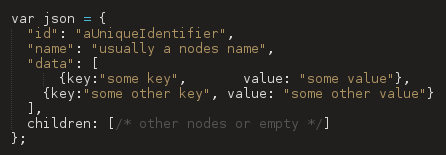
\includegraphics[scale=0.5]{example1.png}
\caption{Example of JSON strucutre}
\end{figure}
\end{center}
\paragraph*{}
\textbf{About datasets:} Sometimes some dataset objects are read by the JIT classes to perform proper layouts. For example, the treemap class reads the first object's value for each node's dataset to perform calculations about the dimensions of the rectangles laid. Also, if you enable the Config.Color.allow property, the treemap will add colors on the layout, and these colors will be based on your second dataset object value. \textbf{RGraphs} and Hyperbolic Trees also read the first dataset object value in order to compute node diameters and angular widths, when setting Config.allowVariableNodeDiameters = true. That's all for now. I recommend you to read the On controllers section and then some spacetree, hypertree, treemap or RGraph tutorials.
\paragraph*{}
\textbf{how to set the RGraph up and running:} the RGraph is inspired by Animated Exploration of Dynamic Graphs with Radial Layout (Ka-Ping Yee, Danyel Fisher, Rachna Dhamija, Marti Hearst) \url{http://bailando.sims.berkeley.edu/papers/infovis01.htm}
This visualization was built and engineered from scratch, taking only the paper as inspiration, and only shares some features with the visualization described in the paper.
Now for the implementation we are going to work with this tree JSON structure: 
\newpage
\begin{figure}[h]
\centering
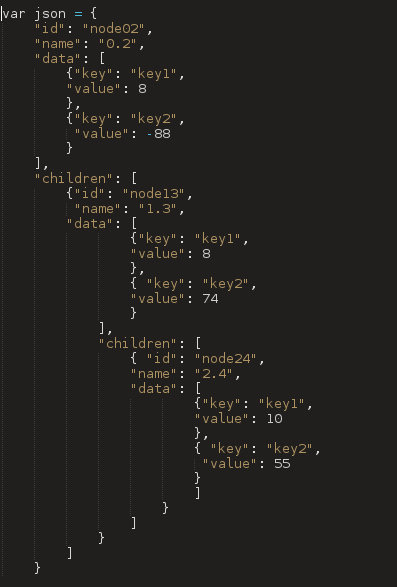
\includegraphics[scale=0.5]{example2.png}
\caption{tree JSON strcuture}
\end{figure}

\paragraph*{}
Put this HTML in your page: 

\begin{figure}[h]
\centering
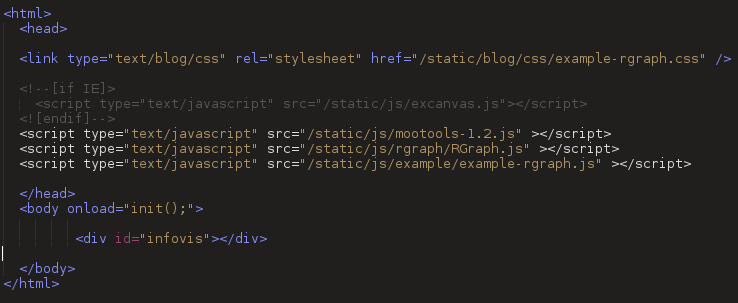
\includegraphics[scale=0.5]{htmlpage.png}
\caption{HTML page}
\end{figure}
\newpage
\paragraph*{}
You'll probably have to change the paths to the css and javascript files. Now, create a rgraph-example.css and put this code in it:

\begin{figure}[h]
\centering
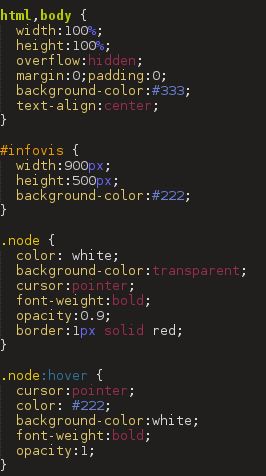
\includegraphics[scale=0.5]{csspage.png}
\caption{CSS RGraph}
\end{figure}

Finally, create an example-rgraph.js file and put this code in it:
\newpage
\begin{figure}[h]
\centering
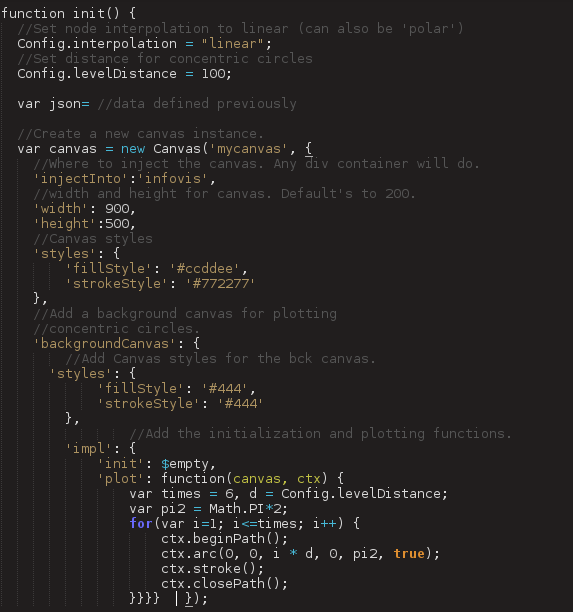
\includegraphics[scale=0.5]{rgraphjs1.png}
\end{figure}
\begin{figure}[h]
\centering
\includegraphics[scale=0.5]{rgraphjs2.png}
\end{figure}
\newpage
\paragraph*{}
You should see a RGraph up and running. Click on the labels and the tree should move. By assigning false to the backgroundCanvas property you can strip off the concentric circles. The backgroundCanvas functions and styles can also be customized to plot whatever background you like. Alsow e can add some JavaScript controller [W16] in order to put the name of the nodes into the labels. We need to use the onCreateLabel method
\begin{figure}[h]
\centering
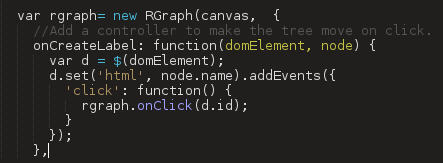
\includegraphics[scale=0.5]{controller.png}
\end{figure}
\paragraph*{}
For more information about the controller on RGraph tools you can visit this API docuementation [W17] created by Nicolas 
\end{document}
